\documentclass{beamer}%
% Choose how your presentation looks.
%
% For more themes, color themes and font themes, see:
% http://deic.uab.es/~iblanes/beamer_gallery/index_by_theme.html
%
\mode<presentation>
{
  \usetheme{default}      % or try Darmstadt, Madrid, Warsaw, ...
  \usecolortheme{beaver} % or try albatross, beaver, crane, ...
  \usefonttheme{default}  % or try serif, structurebold, ...
  \usefonttheme[onlymath]{serif}
  \setbeamertemplate{navigation symbols}{}
  \setbeamertemplate{caption}[numbered]
}

\setlength{\belowcaptionskip}{-10pt}

\usepackage[english]{babel}
\usepackage[utf8x]{inputenc}
\usepackage{mathtools}
\usepackage{tikz}

\newcommand\indx[2]{\genfrac{}{}{0pt}{1}{#1}{#2}}
\newcommand\indxx[2]{#1#2}
\newcommand\indxxx[2]{\genfrac{}{}{0pt}{0}{#1}{#2}}

\newcommand\paren[1]{\biggl(#1\biggr)}
\newcommand\set[1]{\left\{#1\right\}}

\title{Counting structures on the $n \times k$ grid graph}
\author{Peter Kagey}
\institute{University of Southern California}
\date[]{
  Graduate Student Combinatorics Conference\\
  April 2019
}

\begin{document}
\begin{frame}
  \titlepage
\end{frame}

% Uncomment these lines for an automatically generated outline.
%\begin{frame}{Outline}
%  \tableofcontents
%\end{frame}

\begin{frame}{Commodore 64 (1/3)} % https://www.youtube.com/watch?v=m9joBLOZVEo
  % When I was working in software, I became known for my one-off programming
  % projects, and so when my colleague ran across this video, he sent it to me,
  % and it indeed piqued my curiosity.
  \center{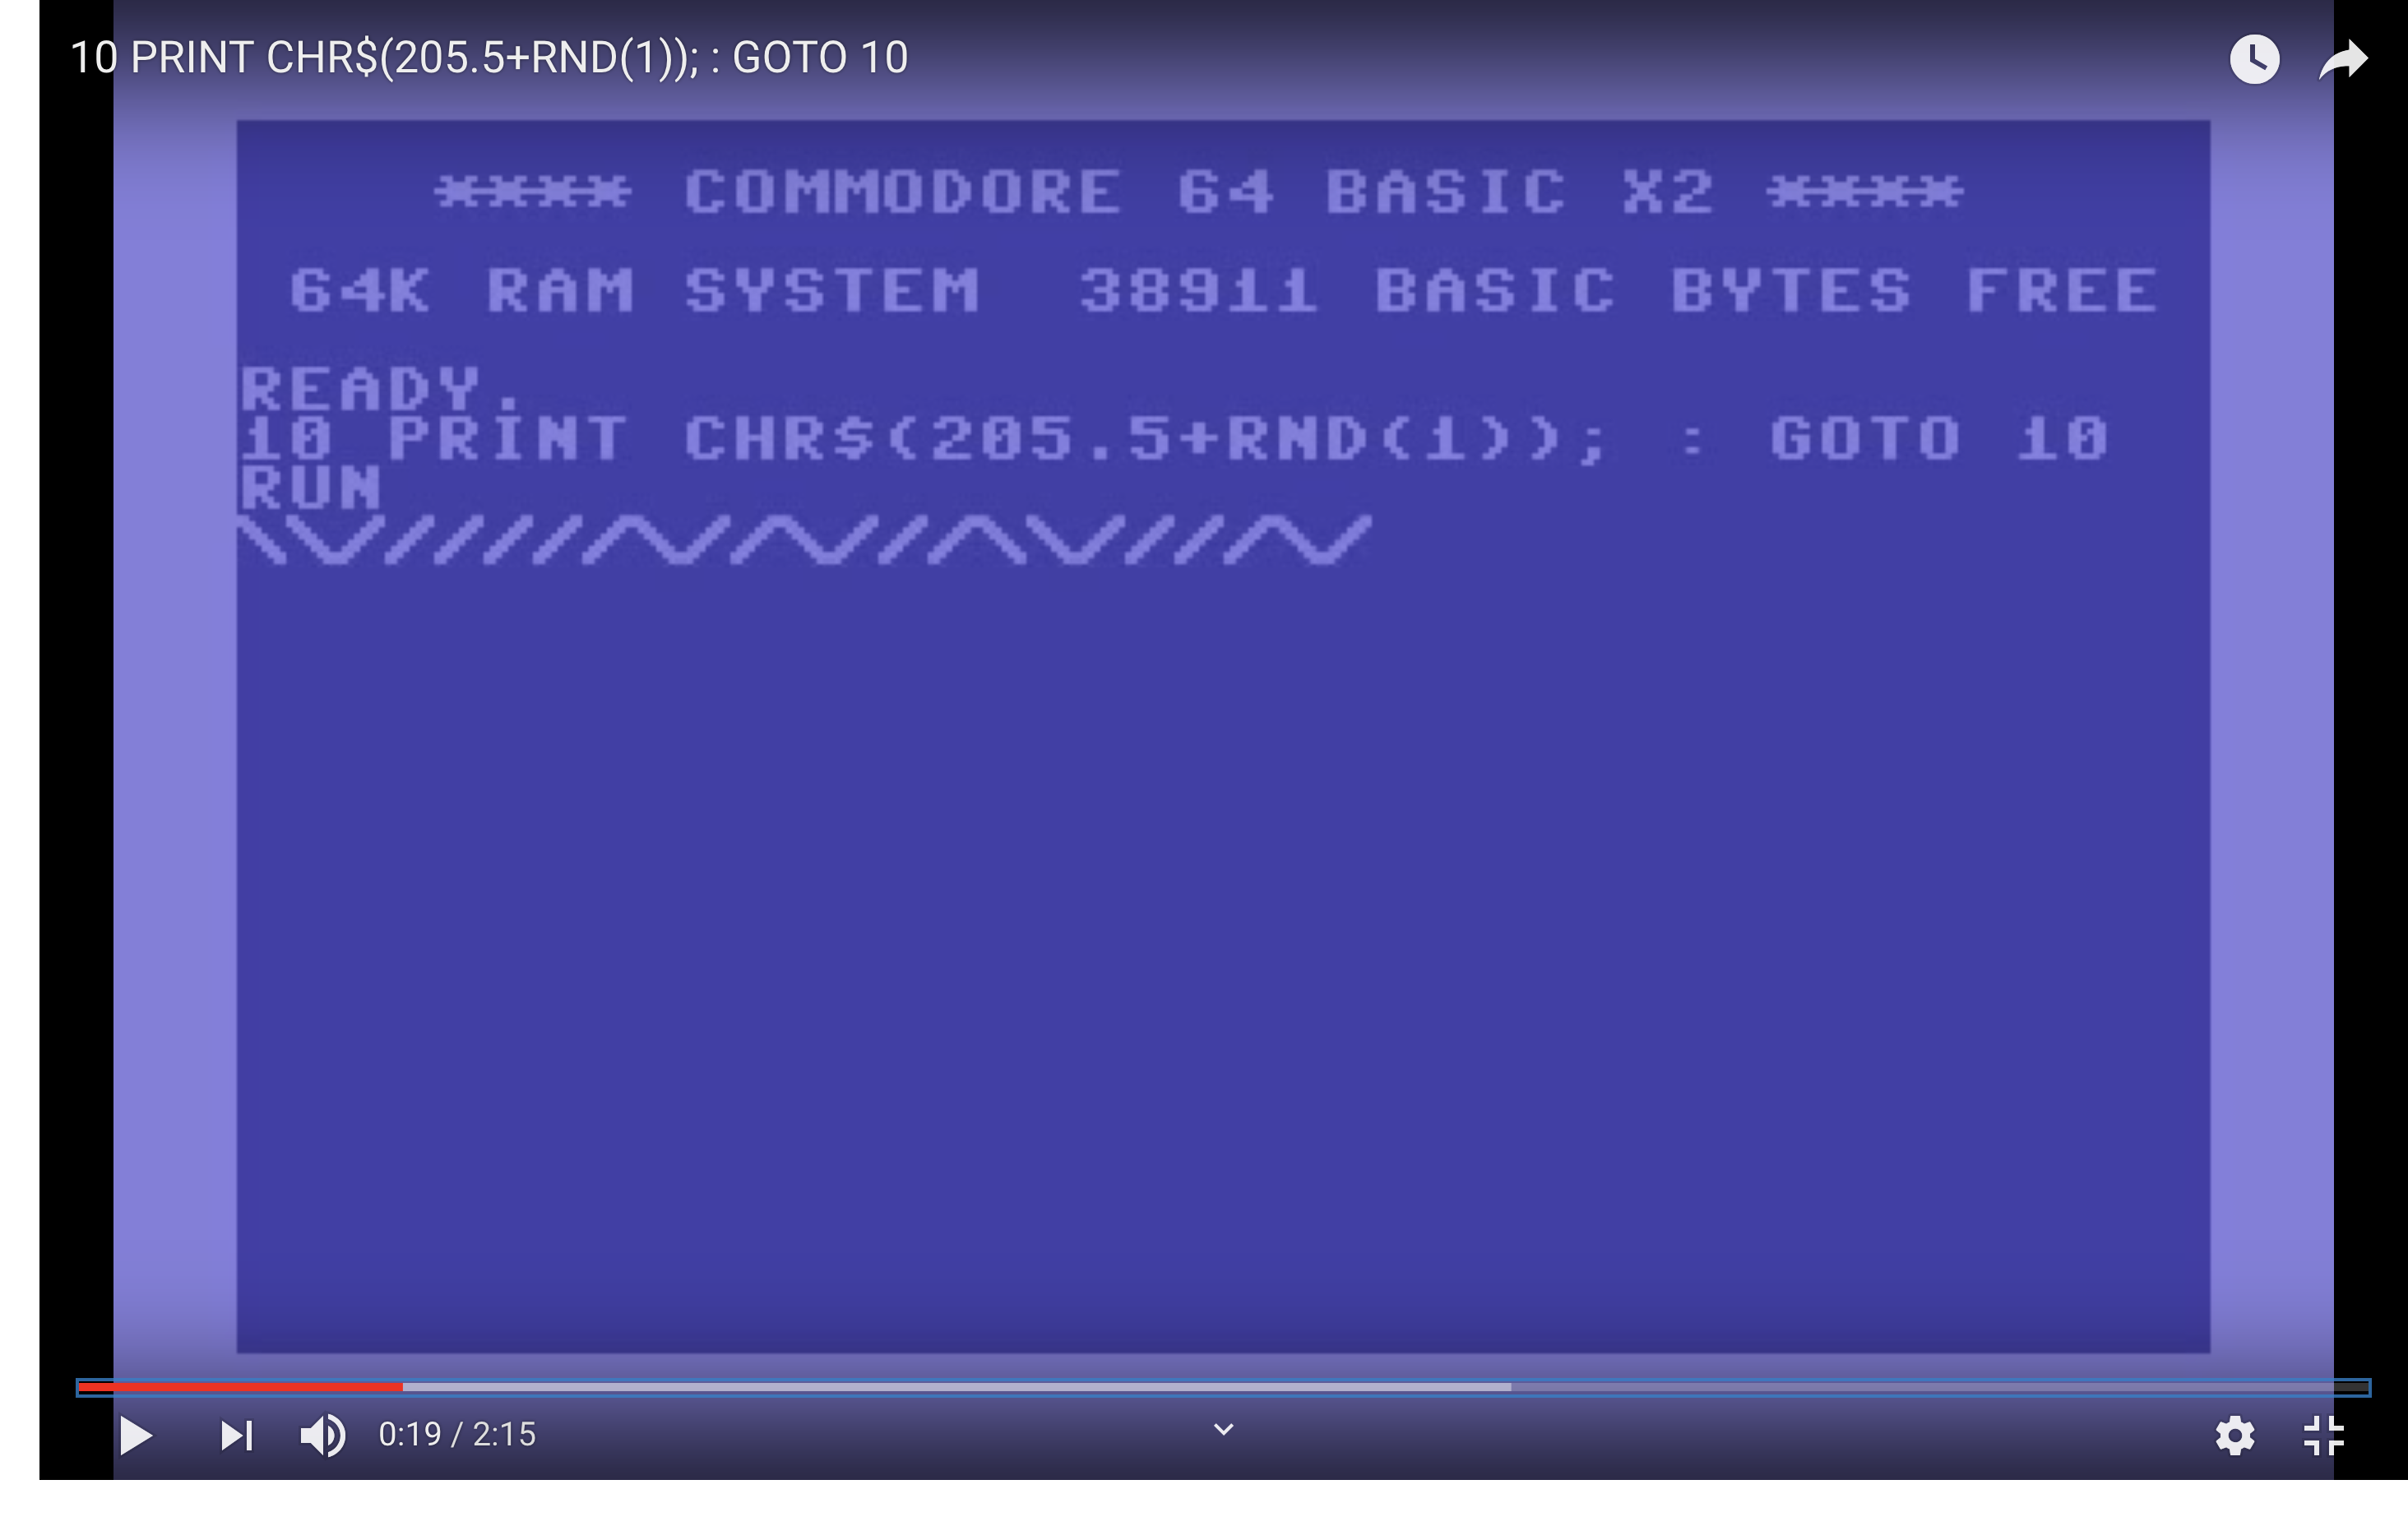
\includegraphics[width=300pt]{commodore64_1.png}}
\end{frame}

\begin{frame}{Commodore 64 (2/3)} % https://www.youtube.com/watch?v=m9joBLOZVEo
  \center{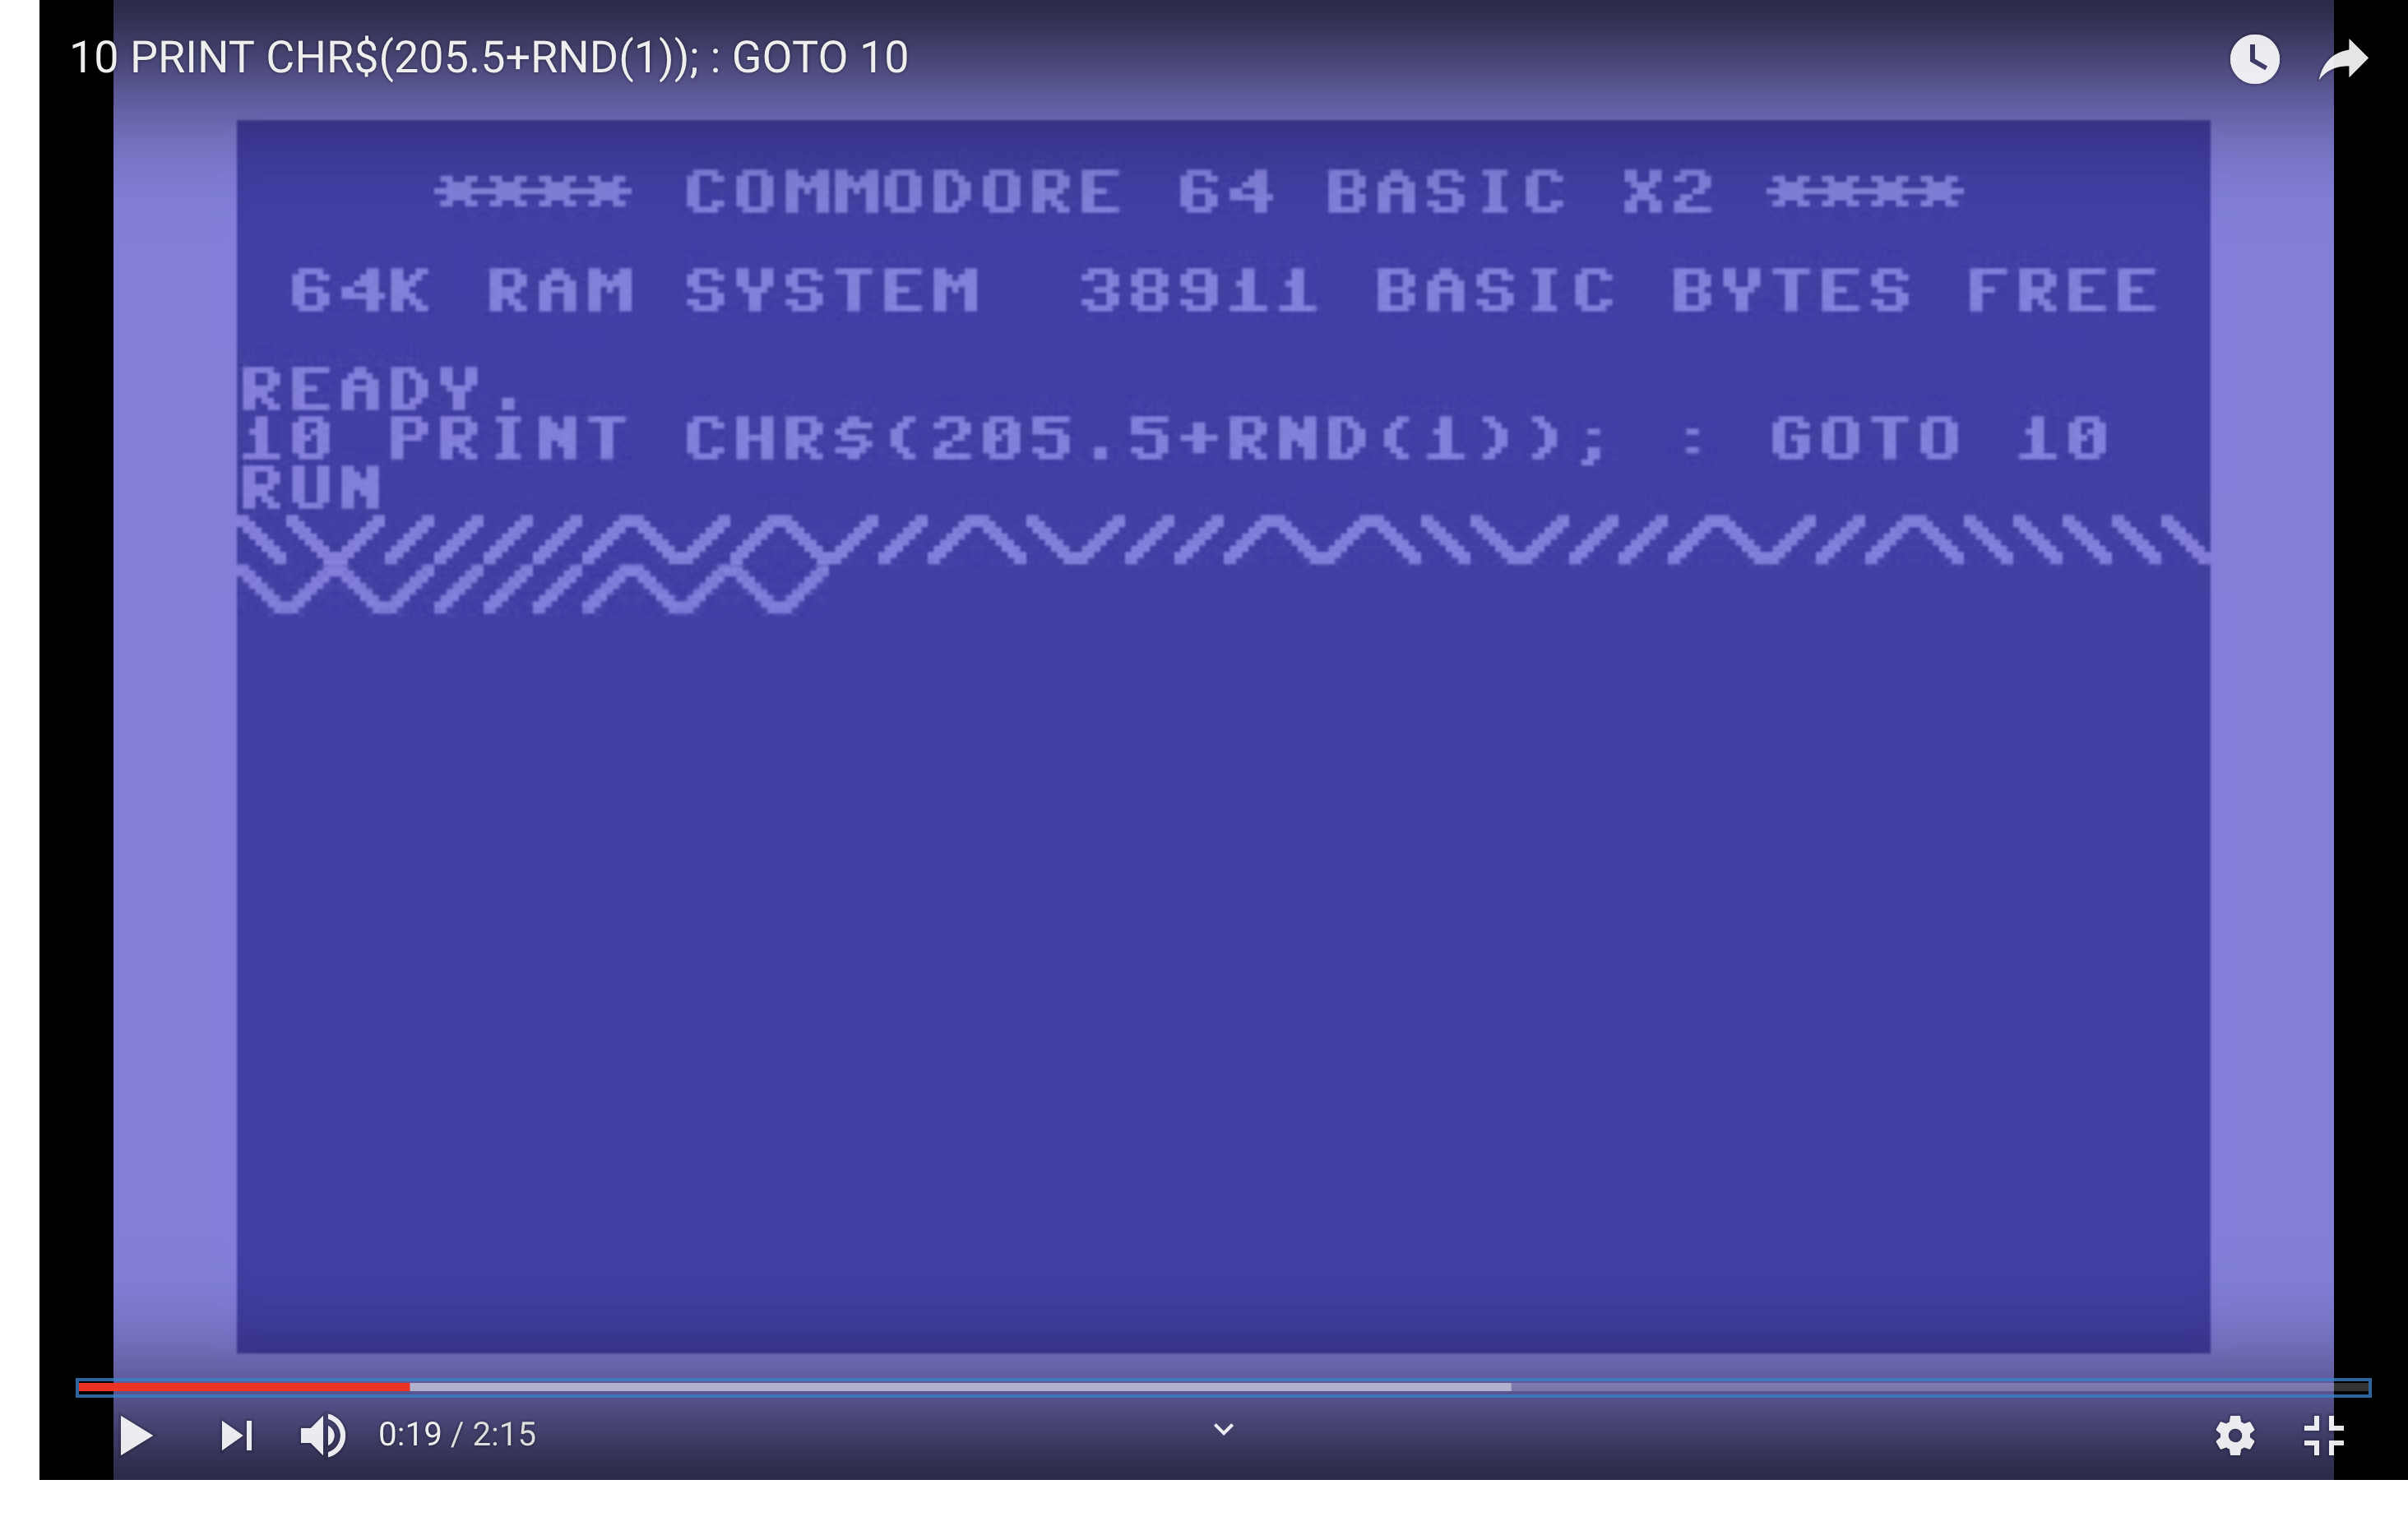
\includegraphics[width=300pt]{commodore64_2.png}}
\end{frame}

\begin{frame}{Commodore 64 (3/3)} % https://www.youtube.com/watch?v=m9joBLOZVEo
  \center{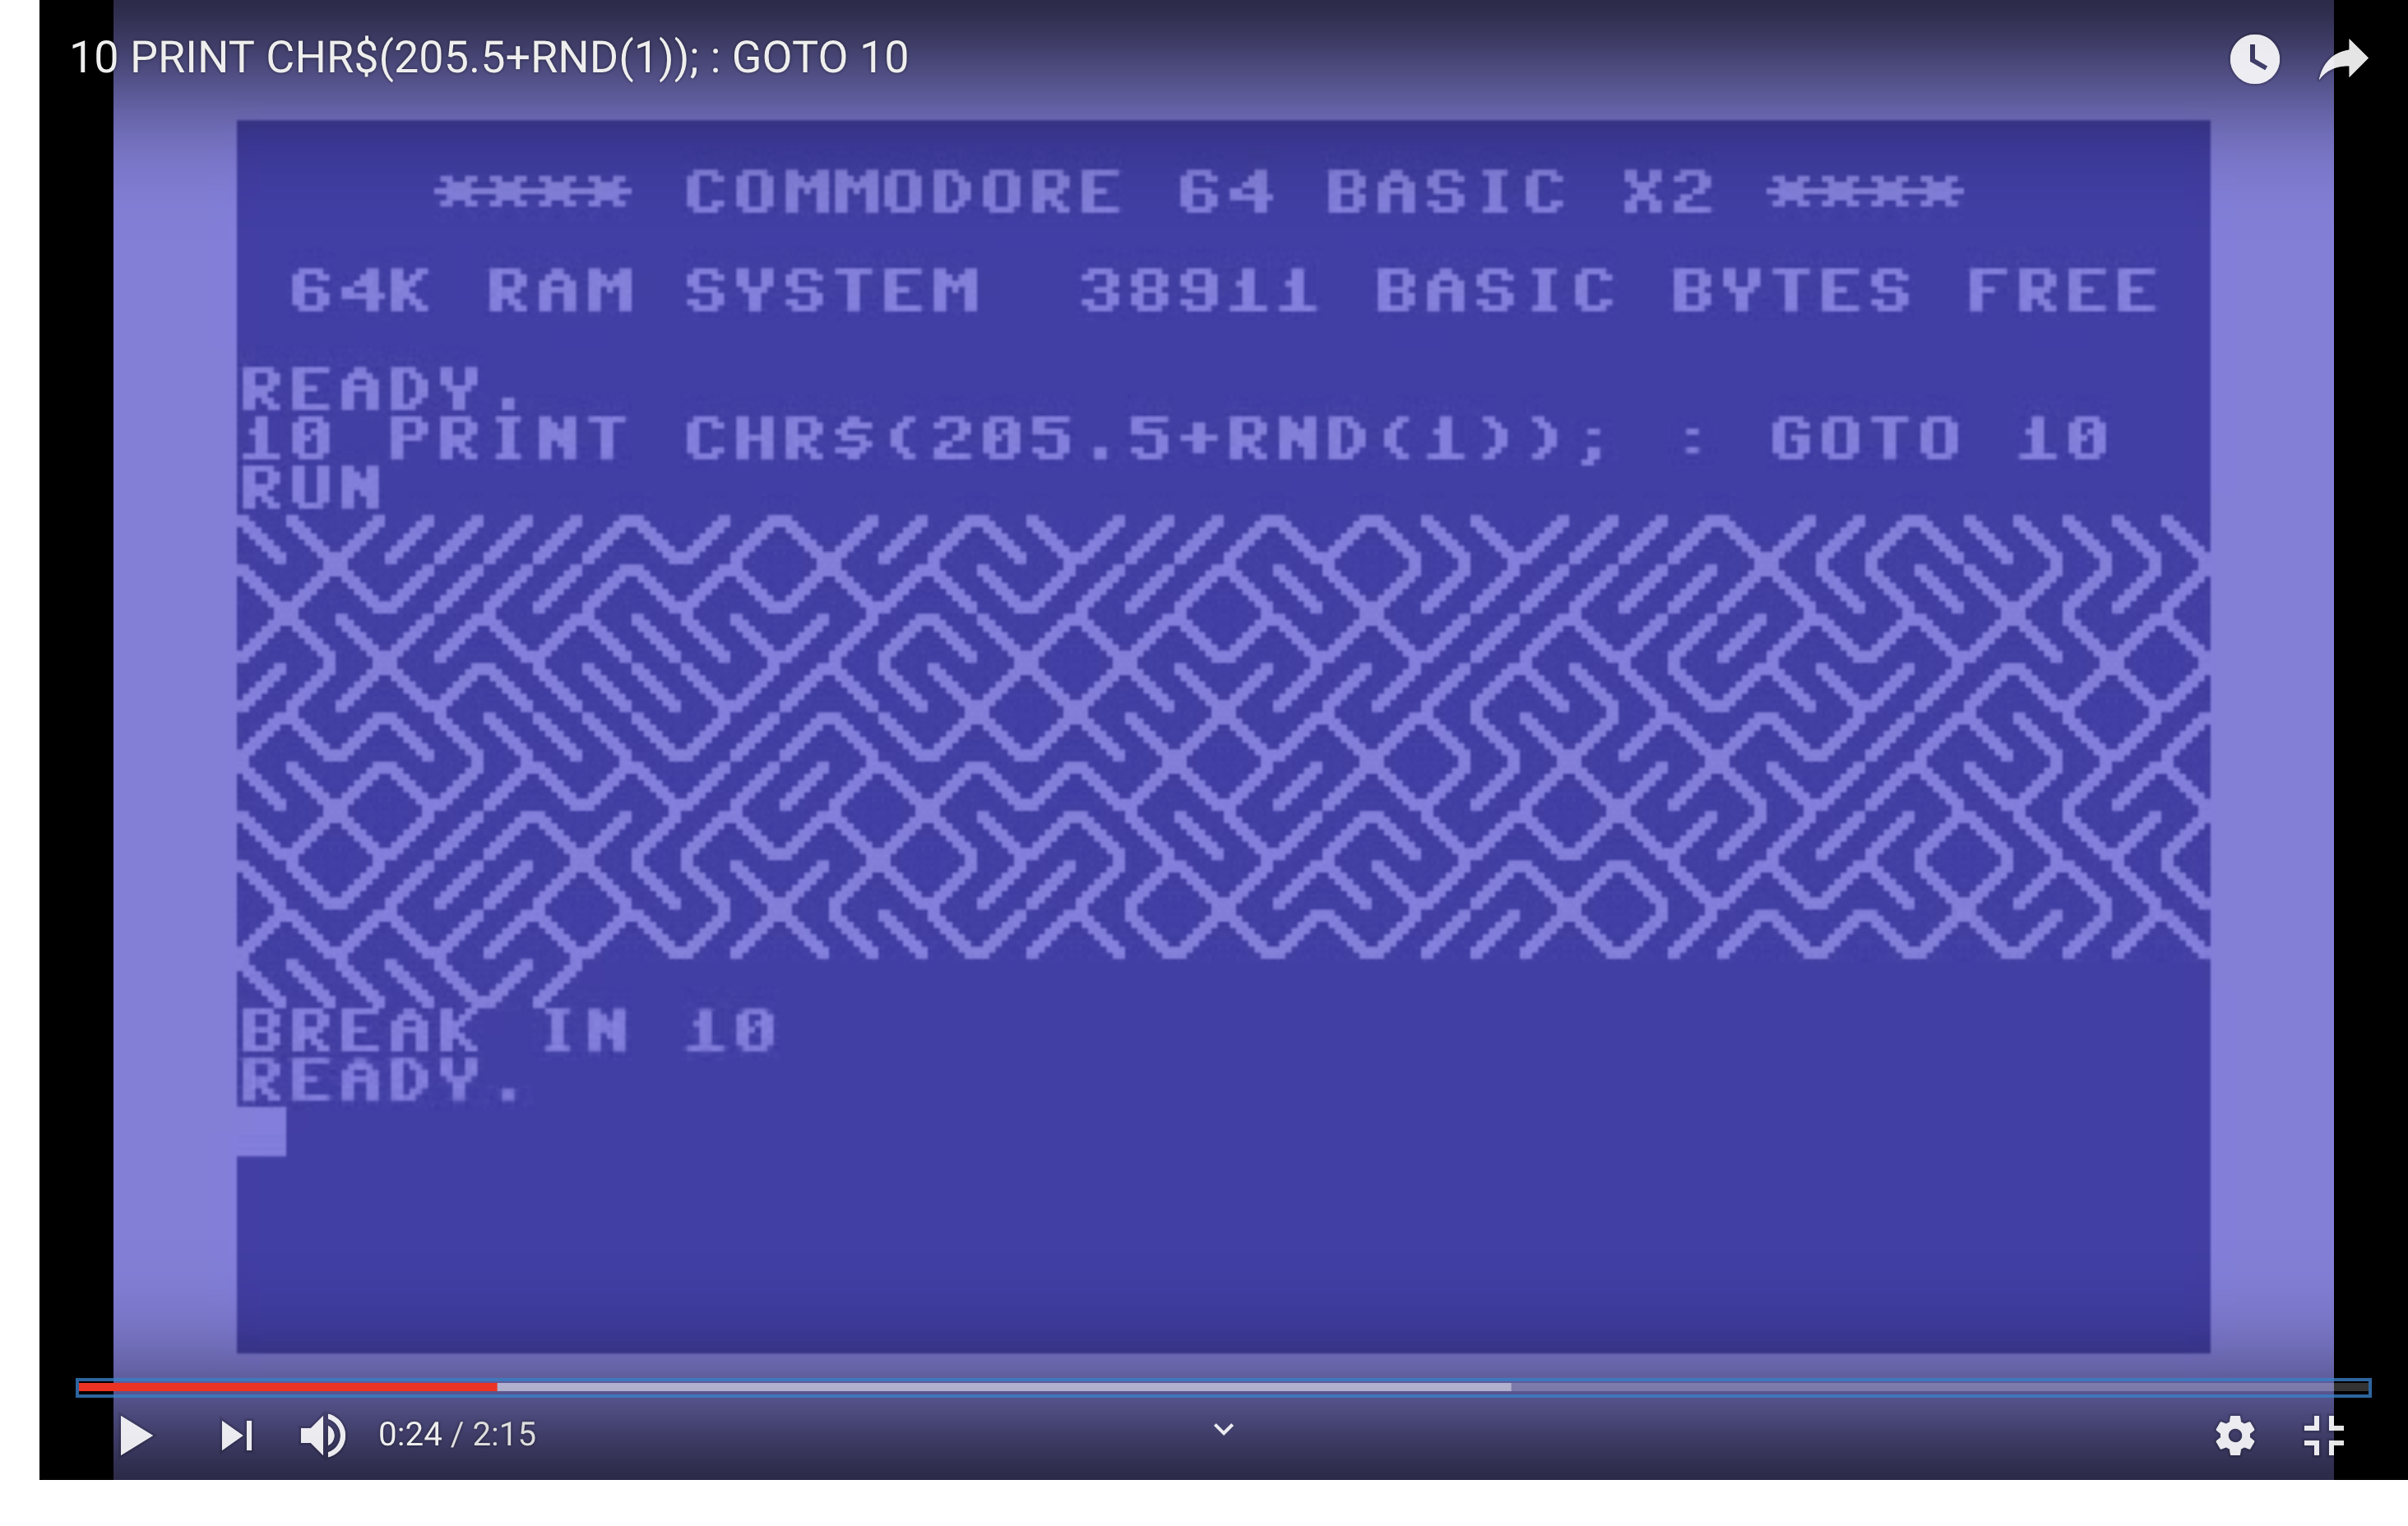
\includegraphics[width=300pt]{commodore64_3.png}}
\end{frame}

\begin{frame}{Javascript} % https://www.youtube.com/watch?v=m9joBLOZVEo
  \center{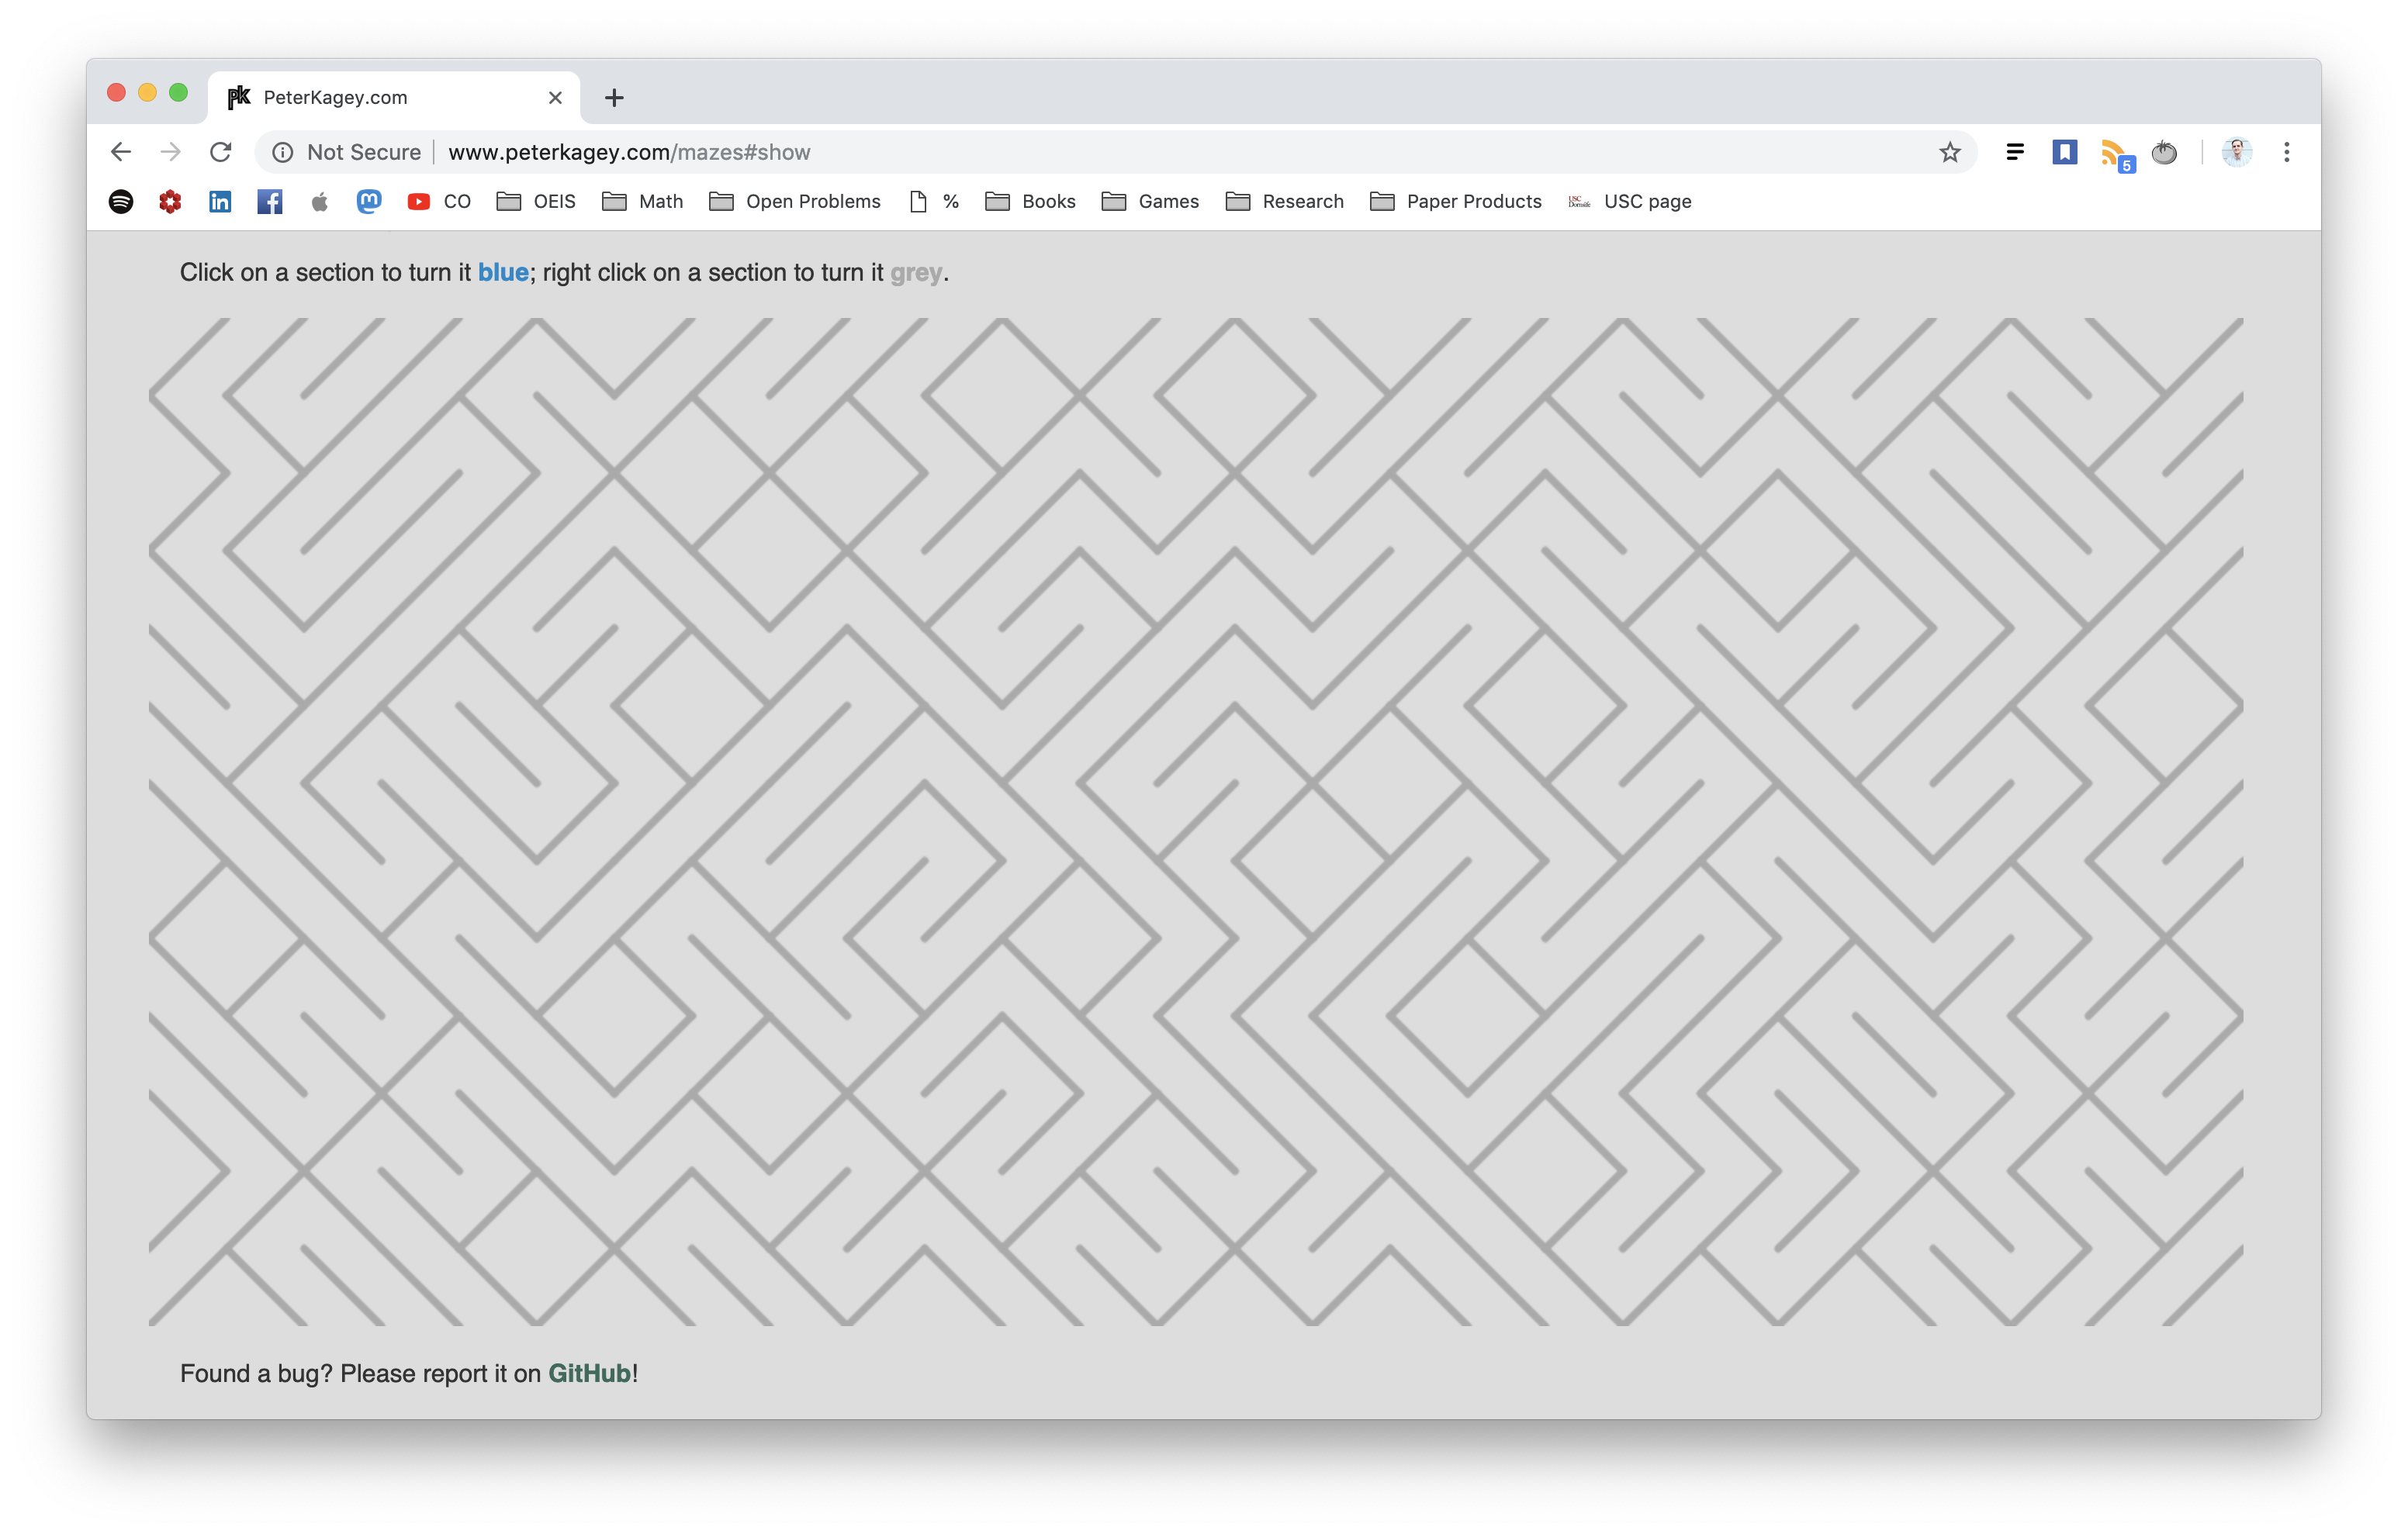
\includegraphics[width=300pt]{website_pre.png}}
\end{frame}

\begin{frame}{Javascript} % https://www.youtube.com/watch?v=m9joBLOZVEo
  \center{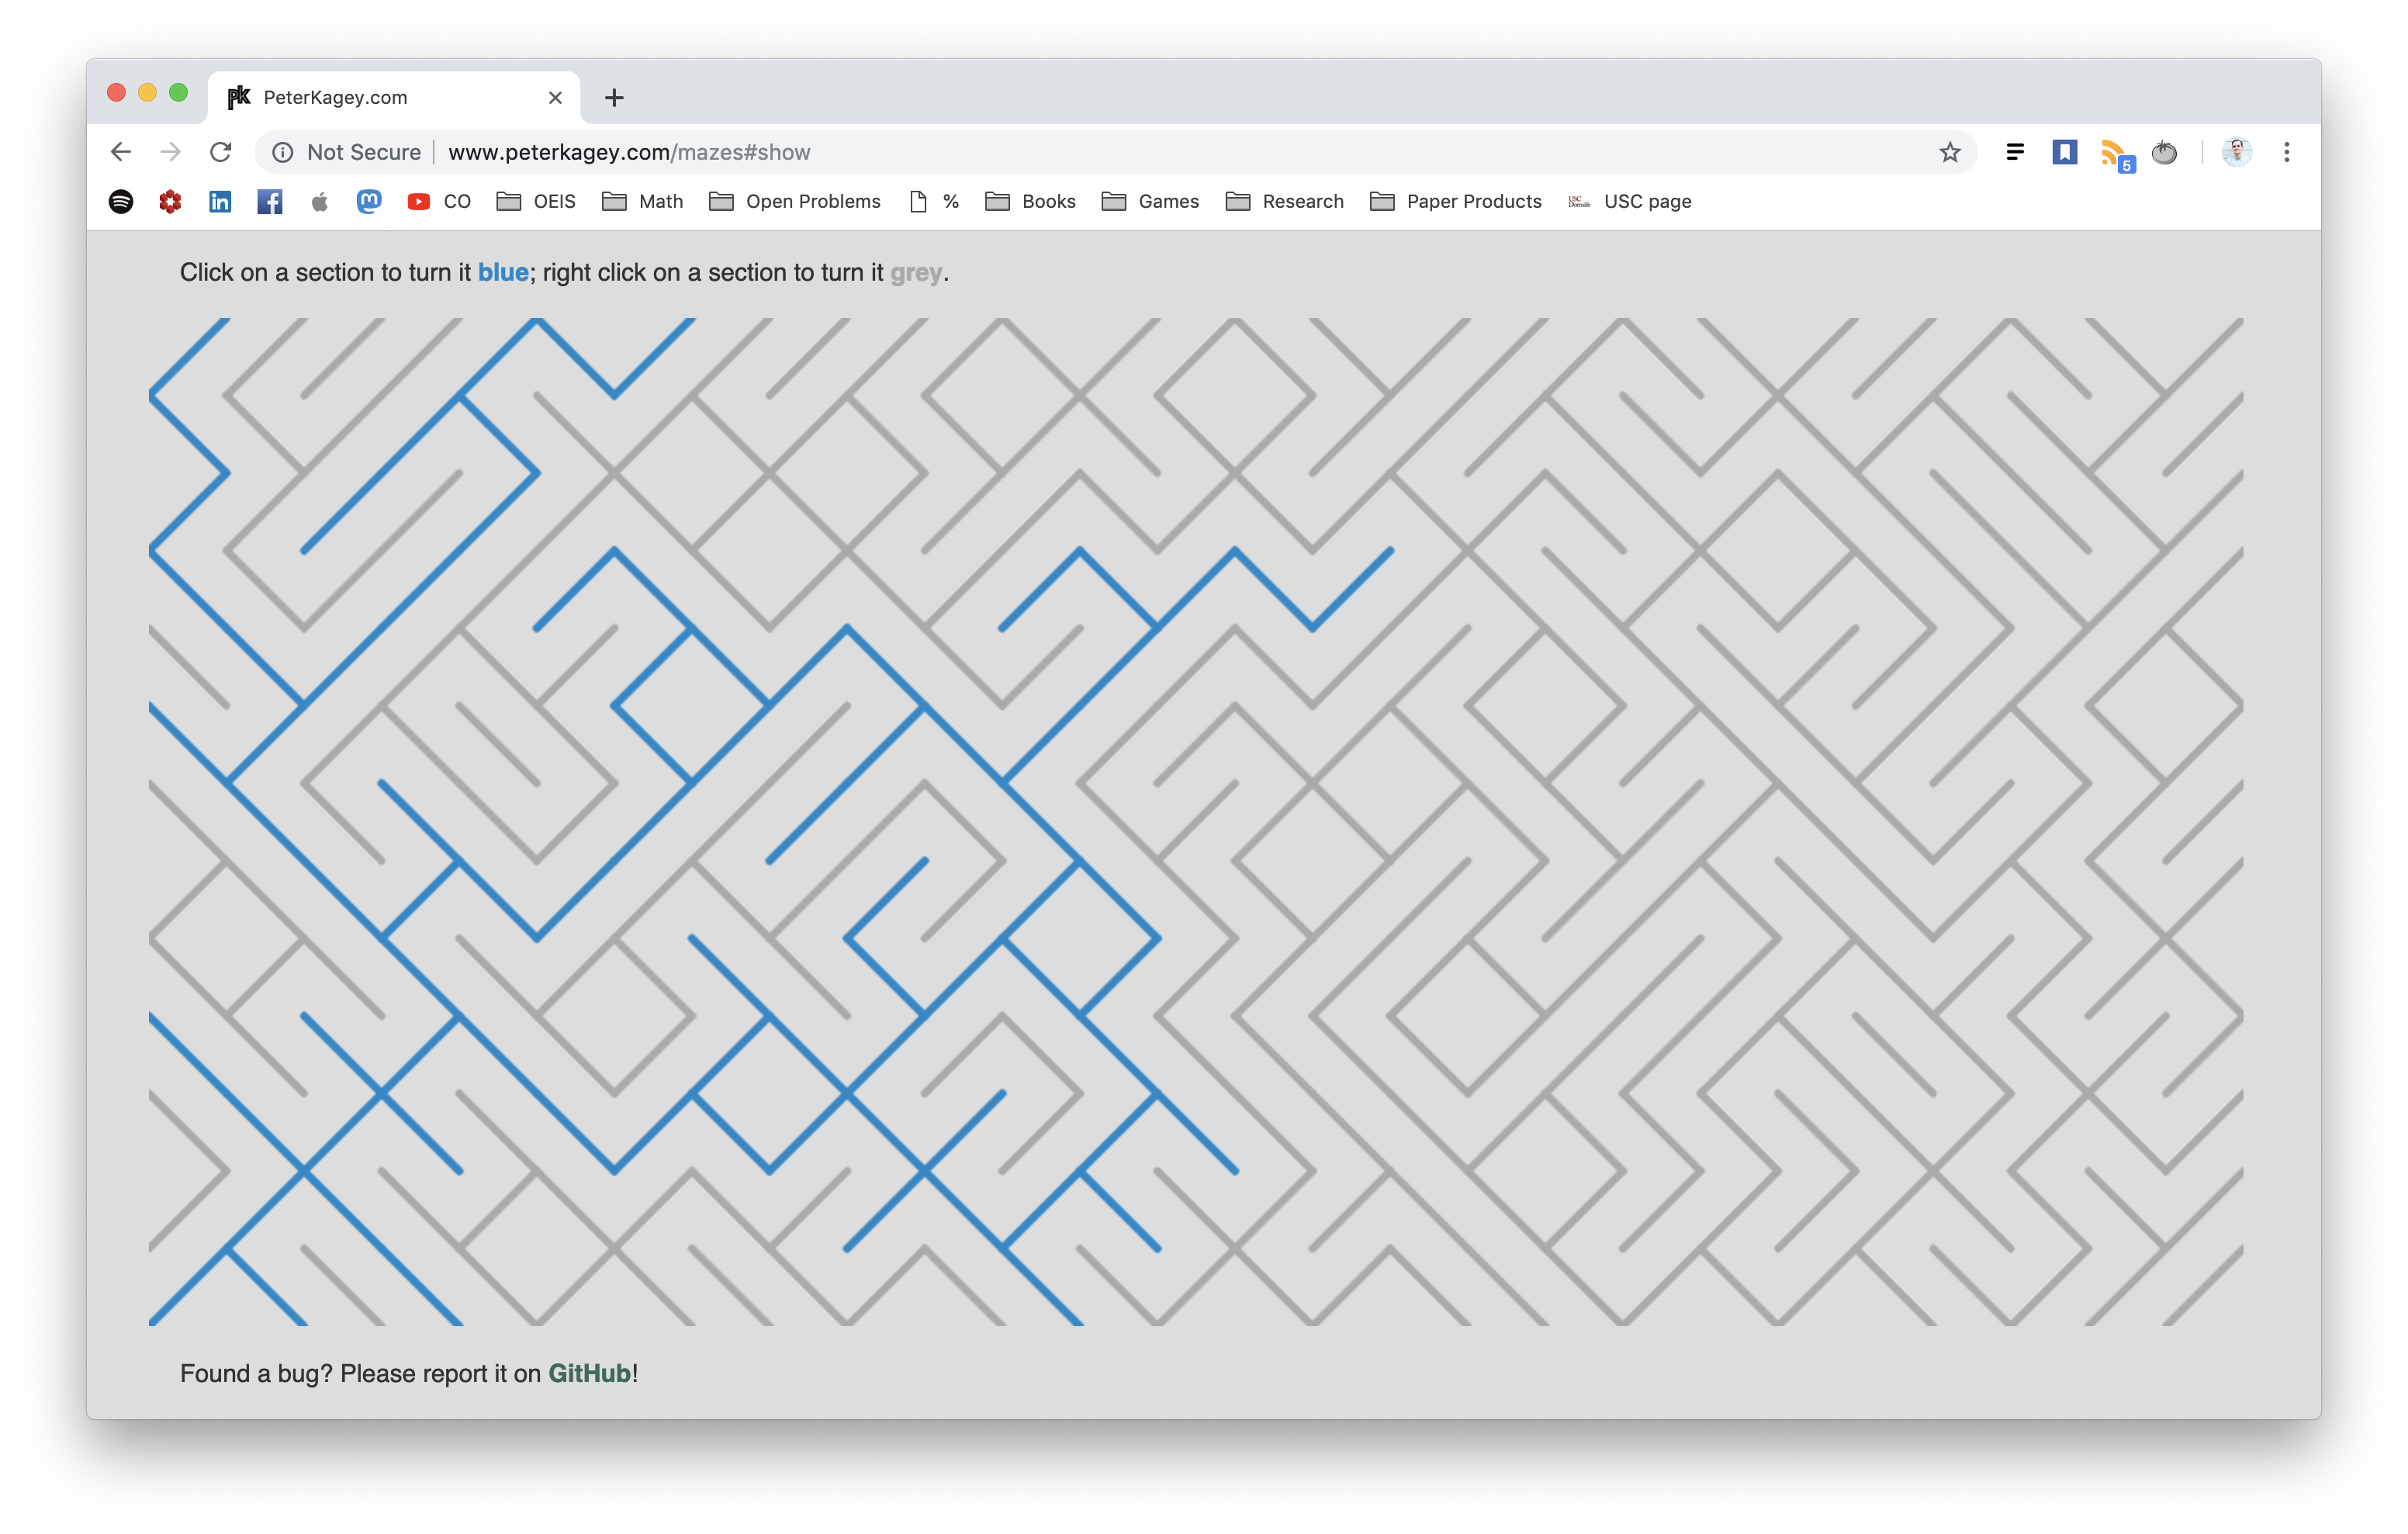
\includegraphics[width=300pt]{website_post.png}}
\end{frame}

\begin{frame}{Counting grids} % V2 Problem 56.
  \begin{figure}
    \begin{center}
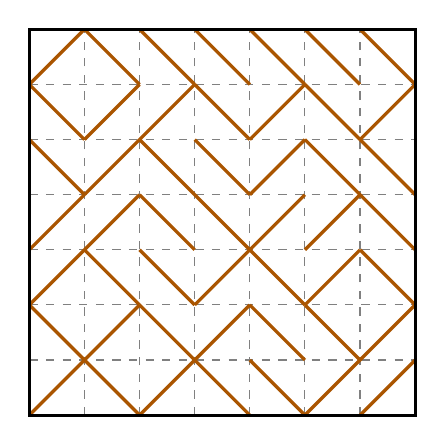
\begin{tikzpicture}[scale=0.7]
  \draw[gray, dashed] (0,0) grid (7,7);
  \foreach \a/\b/\s in {
    0/0/1, 0/1/0, 0/2/1, 0/3/1, 0/4/0, 0/5/0, 0/6/1,
    1/0/0, 1/1/1, 1/2/0, 1/3/1, 1/4/1, 1/5/1, 1/6/0,
    2/0/1, 2/1/0, 2/2/0, 2/3/0, 2/4/0, 2/5/1, 2/6/0,
    3/0/0, 3/1/1, 3/2/1, 3/3/0, 3/4/0, 3/5/0, 3/6/0,
    4/0/0, 4/1/0, 4/2/0, 4/3/1, 4/4/1, 4/5/1, 4/6/0,
    5/0/1, 5/1/0, 5/2/1, 5/3/1, 5/4/0, 5/5/0, 5/6/0,
    6/0/1, 6/1/1, 6/2/0, 6/3/0, 6/4/0, 6/5/1, 6/6/0
  } {
    \draw[very thick, draw={rgb:red,2;green,1;blue,0}] (\a, \b + 1 - \s)--(\a + 1, \b + \s );
  }
  \draw[very thick] (0,0) rectangle (7,7);
\end{tikzpicture}
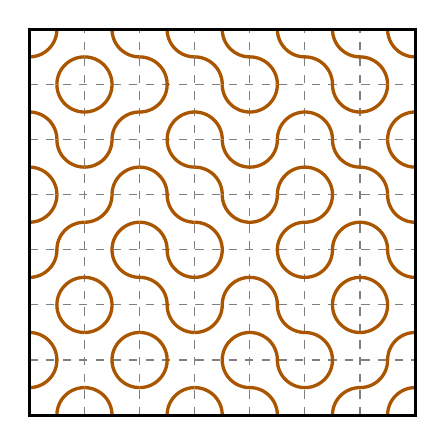
\begin{tikzpicture}[scale=0.7]
  \draw[gray, dashed] (0,0) grid (7,7);
  \foreach \a/\b/\s in {
    0/0/1, 0/1/0, 0/2/1, 0/3/1, 0/4/0, 0/5/0, 0/6/1,
    1/0/0, 1/1/1, 1/2/0, 1/3/1, 1/4/1, 1/5/1, 1/6/0,
    2/0/1, 2/1/0, 2/2/0, 2/3/0, 2/4/0, 2/5/1, 2/6/0,
    3/0/0, 3/1/1, 3/2/1, 3/3/0, 3/4/0, 3/5/0, 3/6/0,
    4/0/0, 4/1/0, 4/2/0, 4/3/1, 4/4/1, 4/5/1, 4/6/0,
    5/0/1, 5/1/0, 5/2/1, 5/3/1, 5/4/0, 5/5/0, 5/6/0,
    6/0/1, 6/1/1, 6/2/0, 6/3/0, 6/4/0, 6/5/1, 6/6/0
  } {
    \draw[very thick, draw={rgb:red,2;green,1;blue,0}, domain=\s*270:\s*270+90]
      plot ({0.5*cos(\x) + \a}, {0.5*sin(\x) + \b + \s});
    \draw[very thick, draw={rgb:red,2;green,1;blue,0}, domain=180-\s*90:270-\s*90]
      plot ({0.5*cos(\x) + \a + 1}, {0.5*sin(\x) + \b  + 1 - \s});
  }
  \draw[very thick] (0,0) rectangle (7,7);
\end{tikzpicture}
\end{center}
    \caption{An illustration of the bijection between tiles with diagonal markings and tiles with quarter circles in opposite corners.}
  \end{figure}
\end{frame}

\begin{frame}{A295229: Number of tilings of the $n \times n$ grid, using diagonal lines to connect the grid points.}
  % A295229
  \begin{figure}[!h]
\centering
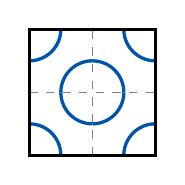
\begin{tikzpicture}[scale=0.8]
  \foreach \a/\b/\theta in {
    0/0/0, 1/1/180,
    1/1/270, 2/0/90,
    0/2/270, 1/1/90,
    1/1/0, 2/2/180} {
    \draw[very thick, draw={rgb:red,0;green,1;blue,2}, domain=\theta:\theta+90] plot ({0.5*cos(\x) + \a}, {0.5*sin(\x) + \b});
  }
  \draw[gray, dashed] (0,0) grid (2,2);
  \draw[very thick] (0,0) rectangle (2,2);
\end{tikzpicture}
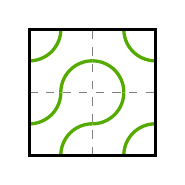
\begin{tikzpicture}[scale=0.8]
  \draw[gray, dashed] (0,0) grid (2,2);
  \foreach \a/\b/\theta in {
    0/1/270, 1/0/90,
    1/1/270, 2/0/90,
    0/2/270, 1/1/90,
    1/1/0, 2/2/180} {
    \draw[very thick, draw={rgb:red,1;green,2;blue,0}, domain=\theta:\theta+90] plot ({0.5*cos(\x) + \a}, {0.5*sin(\x) + \b});
  }
  \draw[very thick] (0,0) rectangle (2,2);
\end{tikzpicture}
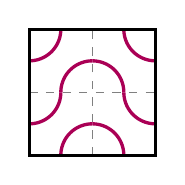
\begin{tikzpicture}[scale=0.8]
  \draw[gray, dashed] (0,0) grid (2,2);
  \foreach \a/\b/\theta in {
    0/1/270, 1/0/90,
    1/0/0, 2/1/180,
    0/2/270, 1/1/90,
    1/1/0, 2/2/180} {
    \draw[very thick, draw={rgb:red,2;green,0;blue,1}, domain=\theta:\theta+90] plot ({0.5*cos(\x) + \a}, {0.5*sin(\x) + \b});
  }
  \draw[very thick] (0,0) rectangle (2,2);
\end{tikzpicture}
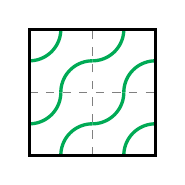
\begin{tikzpicture}[scale=0.8]
  \draw[gray, dashed] (0,0) grid (2,2);
  \foreach \a/\b/\theta in {
    0/1/270, 1/0/90,
    1/1/270, 2/0/90,
    0/2/270, 1/1/90,
    1/2/270, 2/1/90} {
    \draw[very thick, draw={rgb:red,0;green,2;blue,1}, domain=\theta:\theta+90] plot ({0.5*cos(\x) + \a}, {0.5*sin(\x) + \b});
  }
  \draw[very thick] (0,0) rectangle (2,2);
\end{tikzpicture}
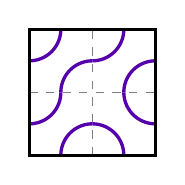
\begin{tikzpicture}[scale=0.8]
  \draw[gray, dashed] (0,0) grid (2,2);
  \foreach \a/\b/\theta in {
    0/1/270, 1/0/90,
    1/0/0, 2/1/180,
    0/2/270, 1/1/90,
    1/2/270, 2/1/90} {
    \draw[very thick, draw={rgb:red,1;green,0;blue,2}, domain=\theta:\theta+90] plot ({0.5*cos(\x) + \a}, {0.5*sin(\x) + \b});
  }
  \draw[very thick] (0,0) rectangle (2,2);
\end{tikzpicture}
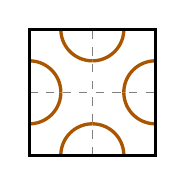
\begin{tikzpicture}[scale=0.8]
  \draw[gray, dashed] (0,0) grid (2,2);
  \foreach \a/\b/\theta in {
    0/1/270, 1/0/90,
    1/0/0, 2/1/180,
    0/1/0, 1/2/180,
    1/2/270, 2/1/90} {
    \draw[very thick, draw={rgb:red,2;green,1;blue,0}, domain=\theta:\theta+90] plot ({0.5*cos(\x) + \a}, {0.5*sin(\x) + \b});
  }
  \draw[very thick] (0,0) rectangle (2,2);
\end{tikzpicture}
\\ \vspace{2pt}
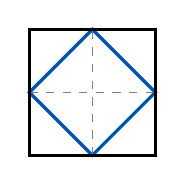
\begin{tikzpicture}[scale=0.8]
  \draw[very thick, draw={rgb:red,0;green,1;blue,2}]
    (0,1)--(1,0)--(2,1)--(1,2)--cycle;
  \draw[gray, dashed] (0,0) grid (2,2);
  \draw[very thick] (0,0) rectangle (2,2);
\end{tikzpicture}
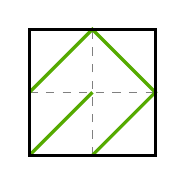
\begin{tikzpicture}[scale=0.8]
  \draw[gray, dashed] (0,0) grid (2,2);
  \draw[very thick, draw={rgb:red,1;green,2;blue,0}]
    (0,0)--(1,1)
    (0,1)--(1,2)--(2,1)--(1,0);
  \draw[very thick] (0,0) rectangle (2,2);
\end{tikzpicture}
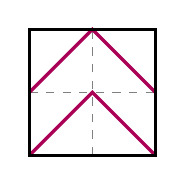
\begin{tikzpicture}[scale=0.8]
  \draw[gray, dashed] (0,0) grid (2,2);
  \draw[very thick, draw={rgb:red,2;green,0;blue,1}]
    (0,0)--(1,1)--(2,0)
    (0,1)--(1,2)--(2,1);
  \draw[very thick] (0,0) rectangle (2,2);
\end{tikzpicture}
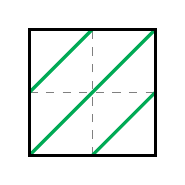
\begin{tikzpicture}[scale=0.8]
  \draw[gray, dashed] (0,0) grid (2,2);
  \draw[very thick, draw={rgb:red,0;green,2;blue,1}]
    (0,1)--(1,2)
    (0,0)--(2,2)
    (1,0)--(2,1);
  \draw[very thick] (0,0) rectangle (2,2);
\end{tikzpicture}
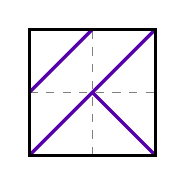
\begin{tikzpicture}[scale=0.8]
  \draw[gray, dashed] (0,0) grid (2,2);
  \draw[very thick, draw={rgb:red,1;green,0;blue,2}]
    (0,1)--(1,2)
    (0,0)--(2,2)
    (1,1)--(2,0);
  \draw[very thick] (0,0) rectangle (2,2);
\end{tikzpicture}
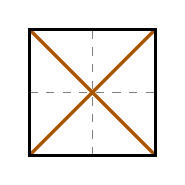
\begin{tikzpicture}[scale=0.8]
  \draw[gray, dashed] (0,0) grid (2,2);
  \draw[very thick, draw={rgb:red,2;green,1;blue,0}]
    (2,0)--(0,2)
    (0,0)--(2,2);
  \draw[very thick] (0,0) rectangle (2,2);
\end{tikzpicture}
\caption {
  An example of the $a(2) = 6$ different ways to fill the $2 \times 2$ grid
  with diagonal tiles up to dihedral action of the square.
}
\end{figure}
  \[
    a(n) = \begin{cases}
      \frac 18 (2^{n^2} + 2\cdot2^{n(n+1)/2} + 3\cdot2^{n^2/2} + 2\cdot2^{n^2/4}) & n \text{ even} \\
      \frac 18 (2^{n^2} + 2\cdot2^{n(n+1)/2} + 2^{(n^2+1)/2}) & n \text{ odd}
    \end{cases}
  \]
  % $1, 6, 84, 8548, 4203520, 8590557312, 70368815480832, \hdots$
\end{frame}

\begin{frame}{Other tiles} % https://www.youtube.com/watch?v=m9joBLOZVEo
    \begin{figure}
      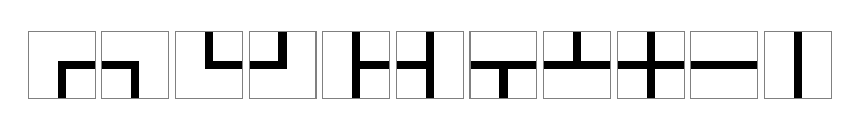
\begin{tikzpicture}[scale = 0.85]
  \draw[line width = 3] (2.1,0.5)--(1.6,0.5)--(1.6,0);
  \draw[gray] (1.1,0) rectangle (2.1,1);

  \draw[line width = 3] (2.2,0.5)--(2.7,0.5)--(2.7,0);
  \draw[gray] (2.2,0) rectangle (3.2,1);

  \draw[line width = 3] (3.8,1)--(3.8,0.5)--(4.3,0.5);
  \draw[gray] (3.3,0) rectangle (4.3,1);

  \draw[line width = 3] (4.9,1)--(4.9,0.5)--(4.4,0.5);
  \draw[gray] (4.4,0) rectangle (5.4,1);

  \draw[line width = 3] (6,0)--(6,1) (6,0.5)--(6.5,0.5);
  \draw[gray] (5.5,0) rectangle (6.5,1);

  \draw[line width = 3] (7.1,0)--(7.1,1) (7.1,0.5)--(6.6,0.5);
  \draw[gray] (6.6,0) rectangle (7.6,1);

  \draw[line width = 3] (7.7,0.5)--(8.7,0.5) (8.2,0.5)--(8.2,0);
  \draw[gray] (7.7,0) rectangle (8.7,1);

  \draw[line width = 3] (8.8,0.5)--(9.8,0.5) (9.3,0.5)--(9.3,1);
  \draw[gray] (8.8,0) rectangle (9.8,1);

  \draw[line width = 3] (9.9,0.5)--(10.9,0.5) (10.4,0)--(10.4,1);
  \draw[gray] (9.9,0) rectangle (10.9,1);

  \draw[line width = 3] (11.0,0.5)--(12.0,0.5);
  \draw[gray] (11,0) rectangle (12,1);

  \draw[line width = 3] (12.6,0)--(12.6,1);
  \draw[gray] (12.1,0) rectangle (13.1,1);
\end{tikzpicture}

      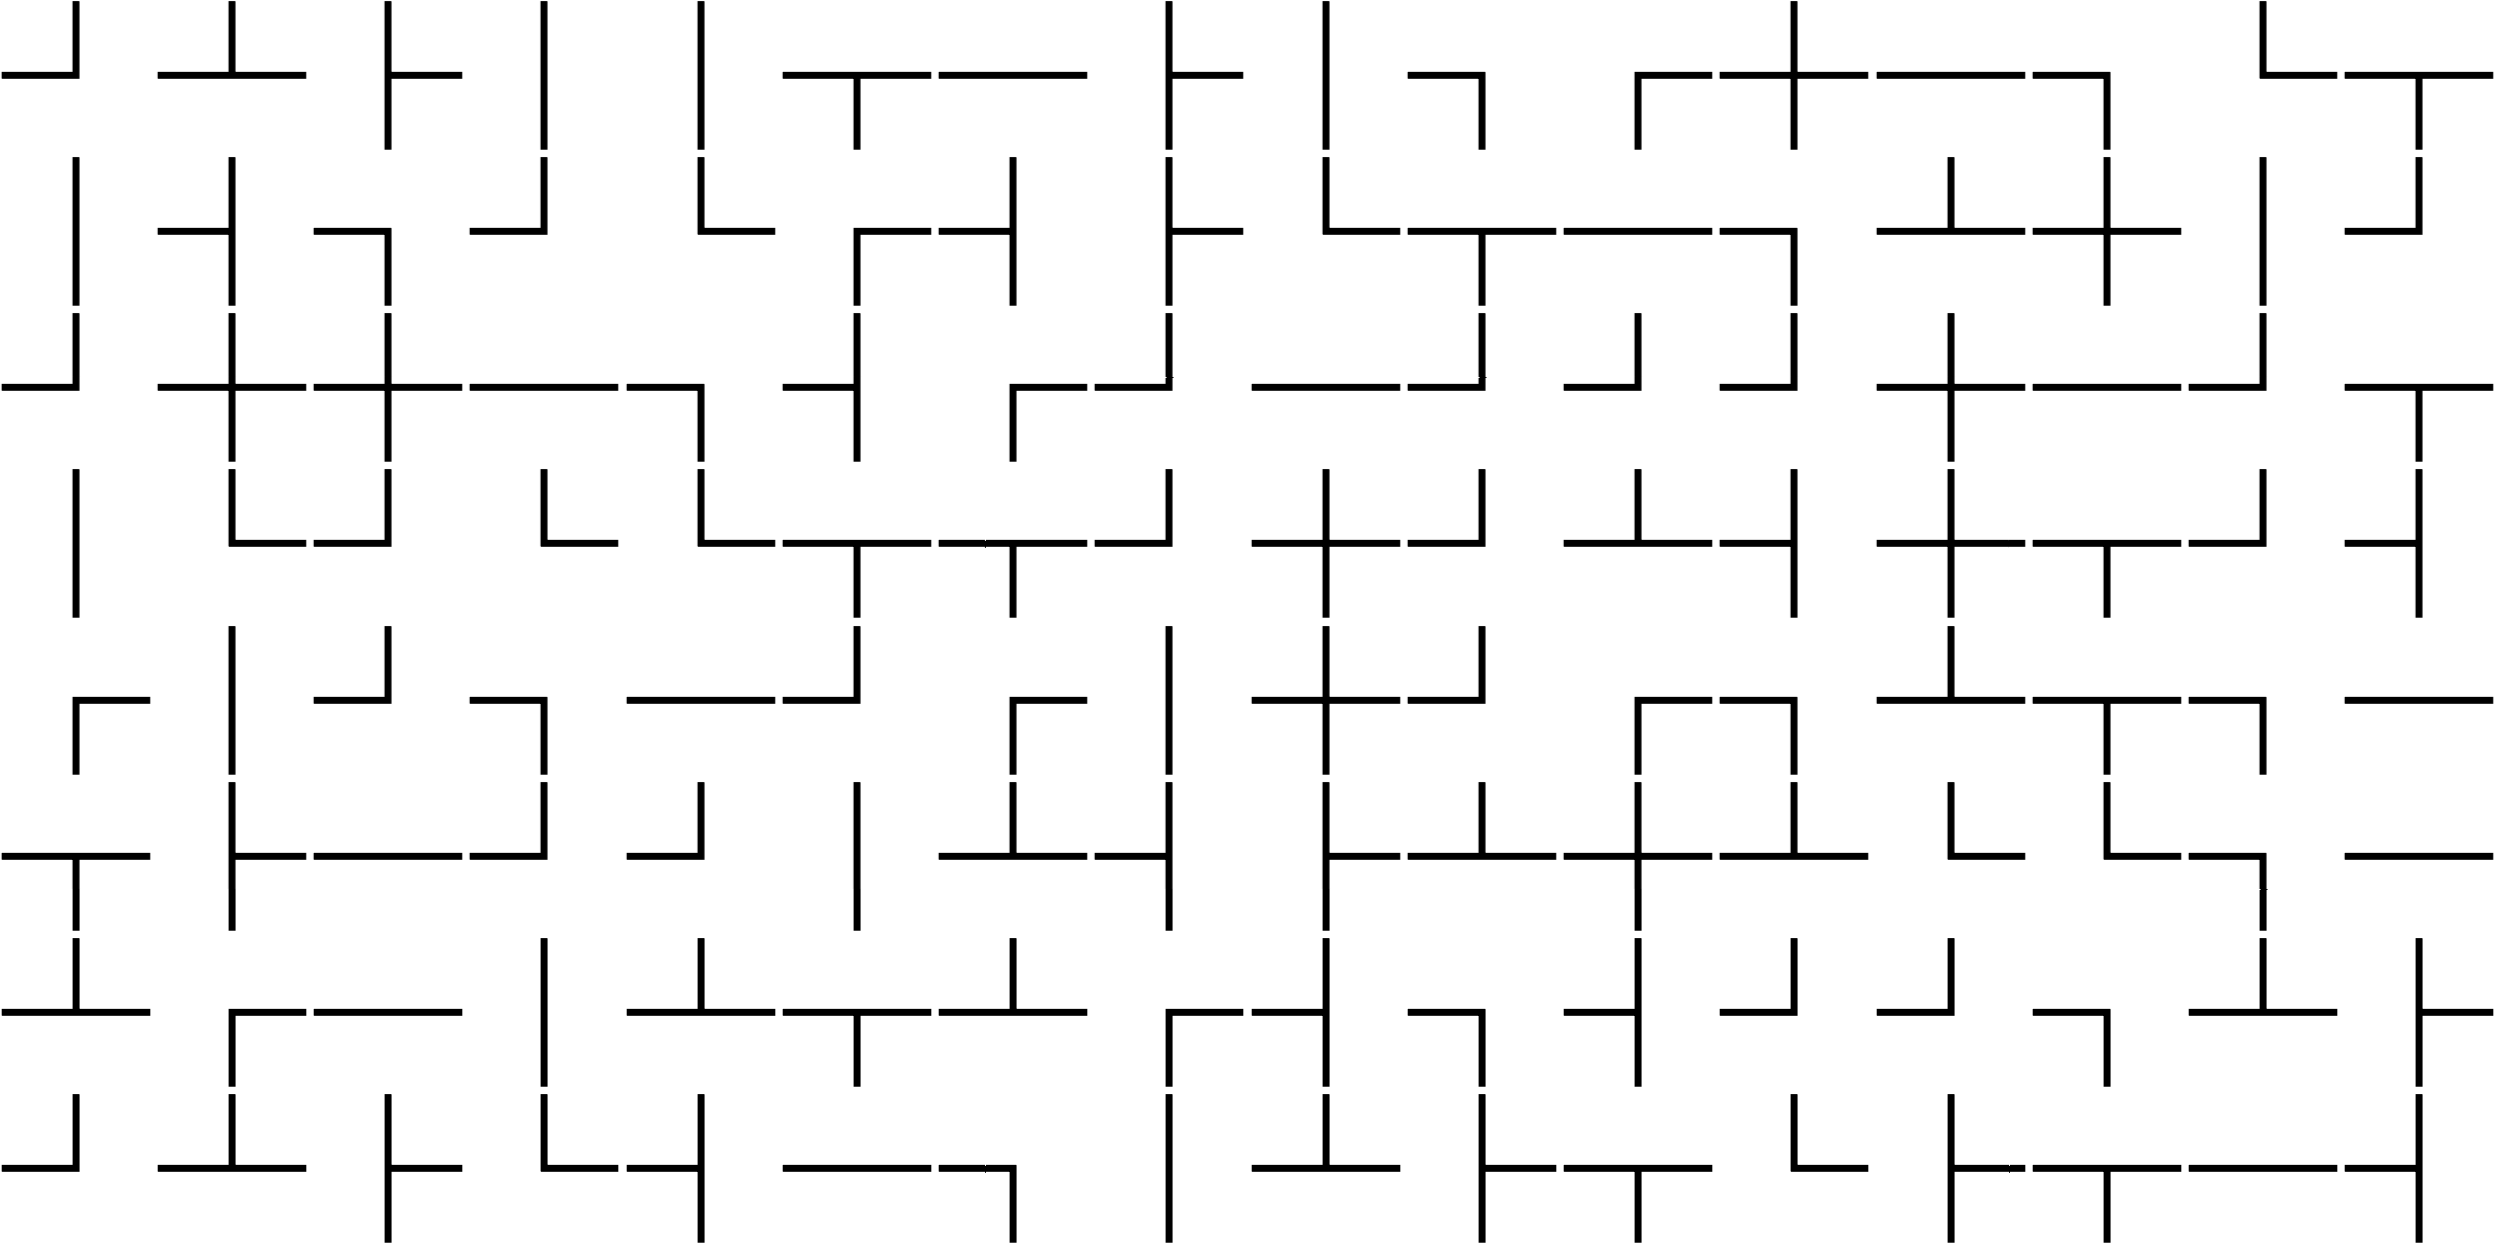
\includegraphics[width=230pt]{pseudomaze2.png}
      \caption{Eleven box-drawing characters placed on an $15 \times 8$ grid}
    \end{figure}
\end{frame}

\begin{frame}{Baby's first corollary}
  \begin{corollary}[of Burnside's Lemma]
    Let \begin{itemize}
      \item $t$ be the number of tiles,
      \item $q$ be the number of tiles symmetric under a $90^\circ$ rotation,
      \item $h$ be the number of tiles symmetric under a $180^\circ$ rotation,
      \item $d$ be the number of tiles symmetric under a diagonal reflection, and
      \item $v$ be the number of tiles symmetric under a vertical reflection.
    \end{itemize}
    Then the number of tilings up to symmetries of the square is
  \[
    a(n) = \begin{cases}
      \frac 18 \paren{
        t^{n^2} + 2qt^{\frac{n^2-1}{4}} + ht^{\frac{n^2-1}{2}} + (v^n + d^n)t^{\frac{n^2-n}{2}}
      } & n \text{ odd} \\
      \\
      \frac 18 \paren{
        t^{n^2} + 3t^{\frac{n^2}{2}} + 2t^{\frac{n^2}{4}} + 2d^n t^{\frac{n^2-n}{2}}
      } & n \text{ even}
    \end{cases}
  \]
  \end{corollary}
\end{frame}

\begin{frame}{Pipe Mania}
  \center{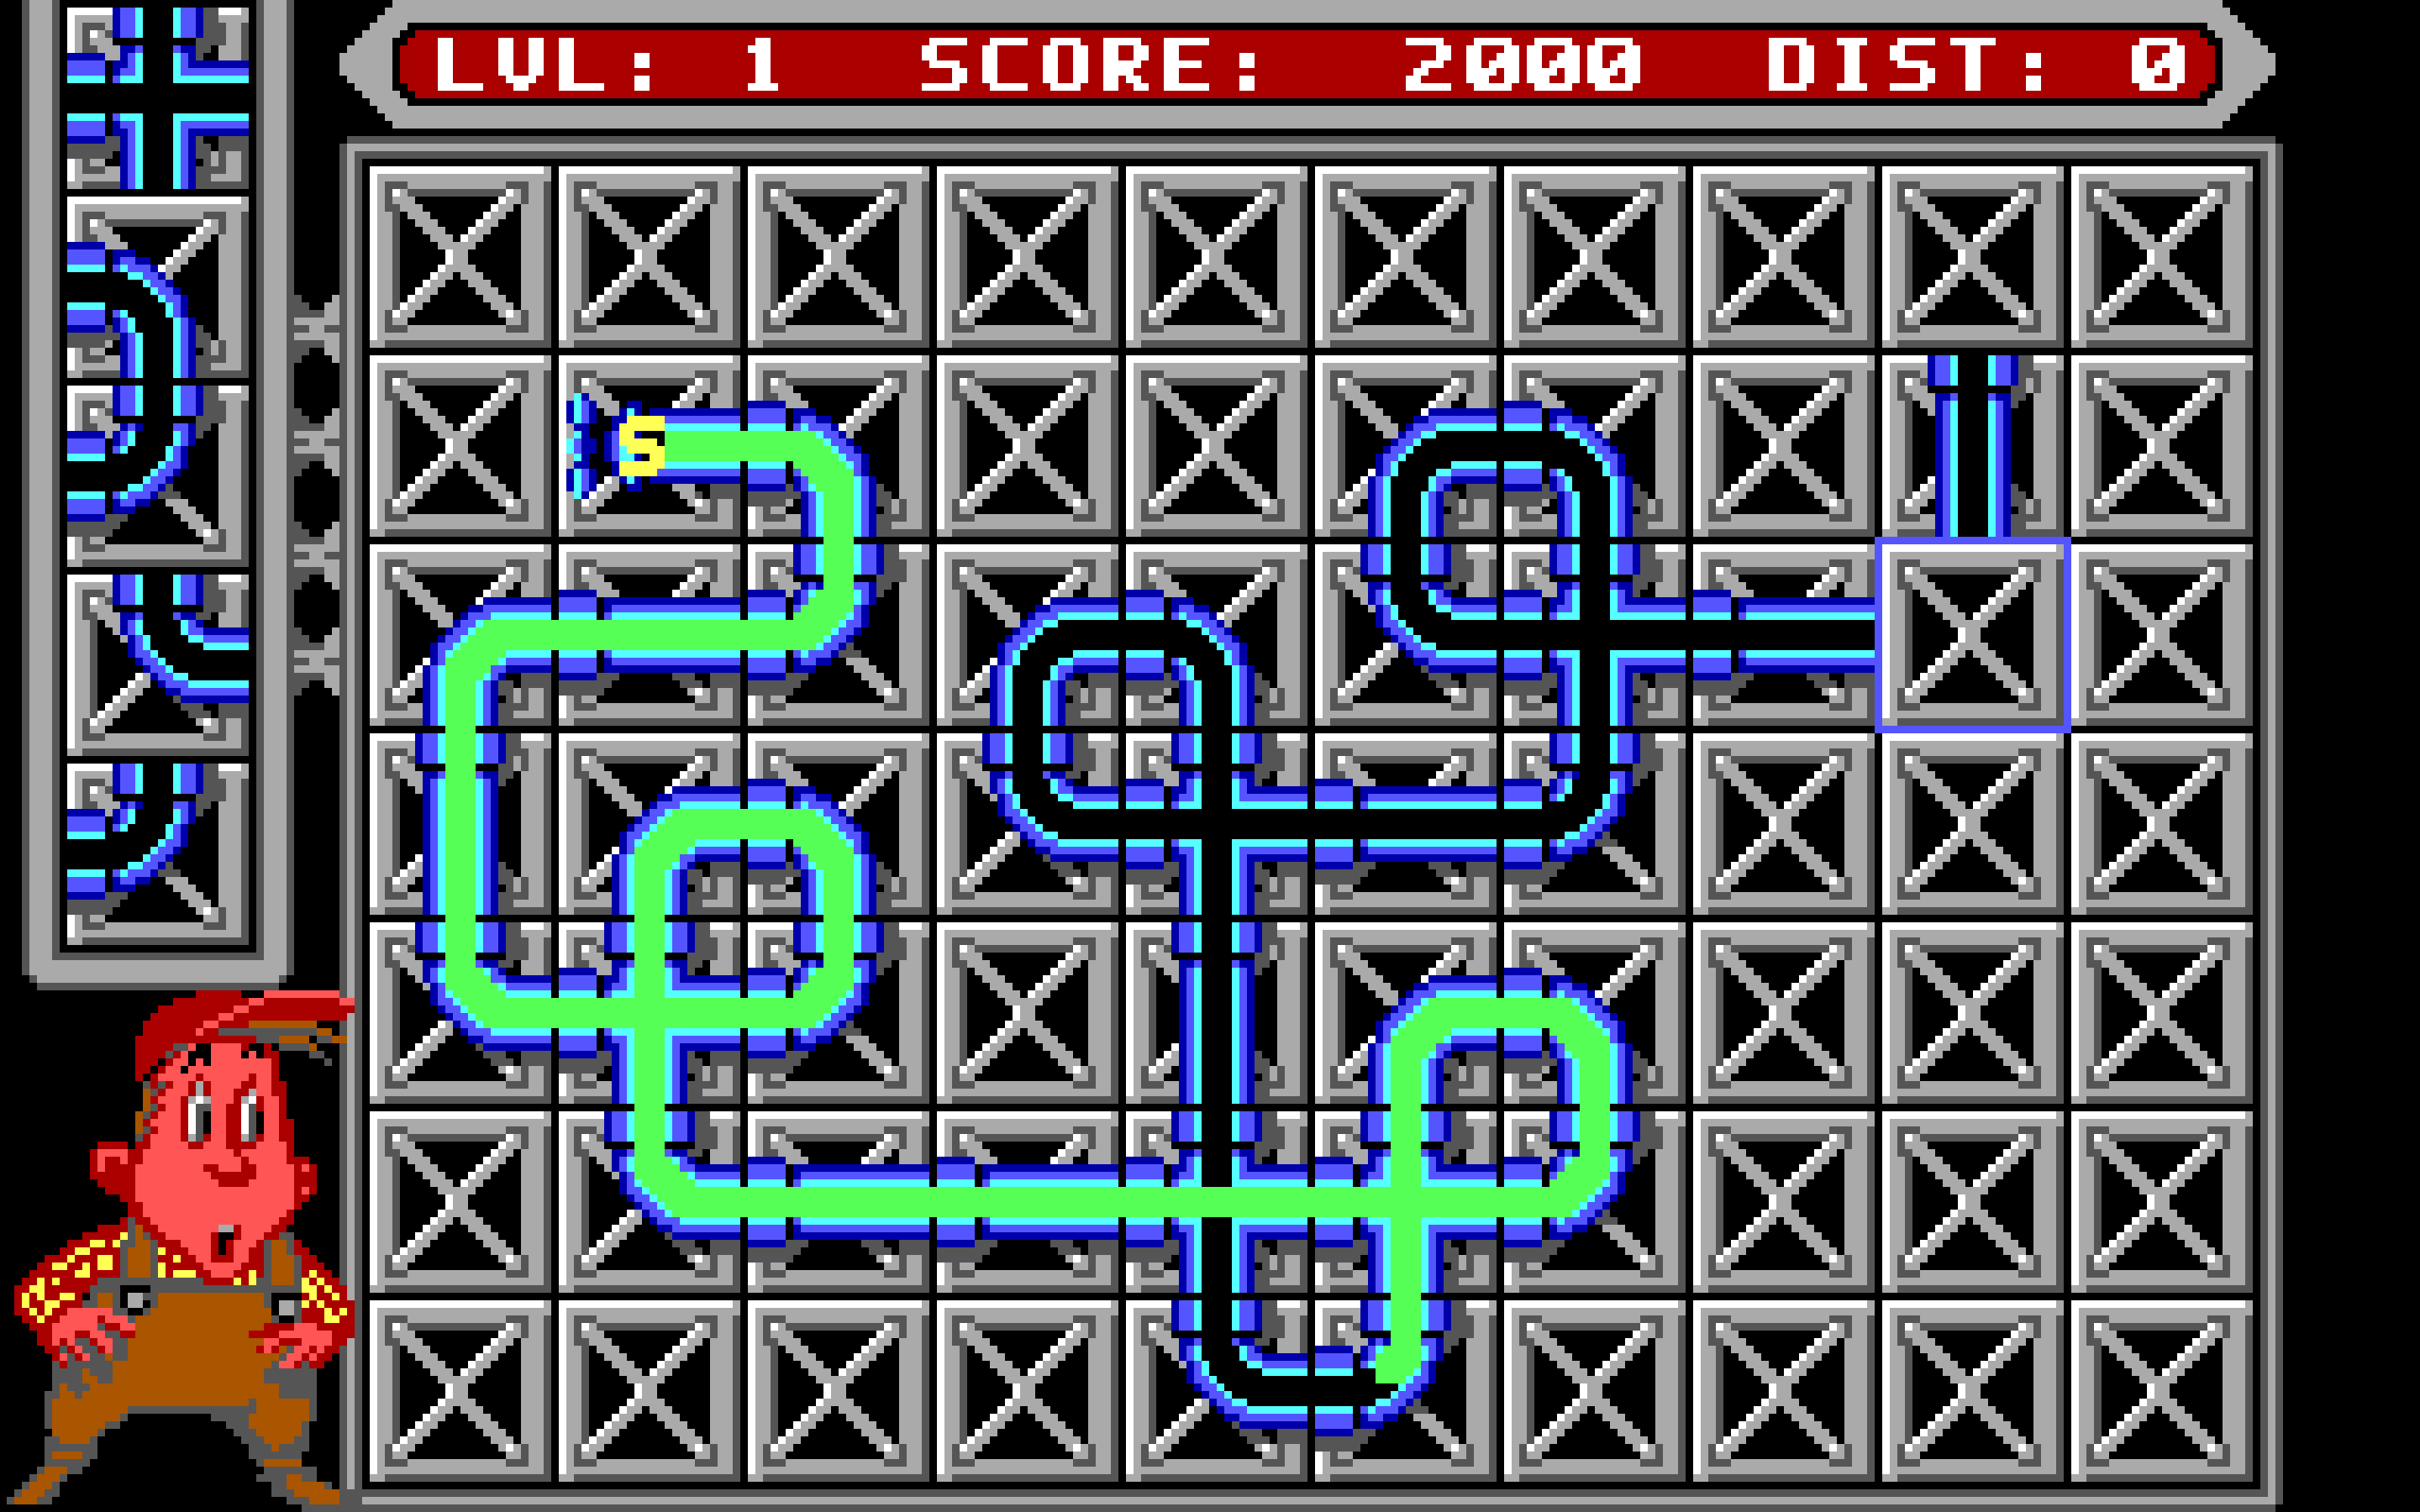
\includegraphics[width=300pt]{pipe_mania.png}}
\end{frame}

\begin{frame}{Leaf-free subgraphs of the grid graph} % V2 Problem 56.
  % Can also use this to count multipartite graphs and planar multipartite graphs.
  \begin{figure}[!h]
    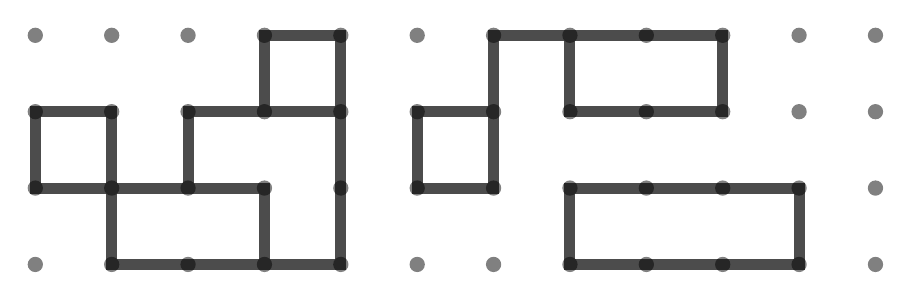
\begin{tikzpicture}[scale=0.97]
  % \draw[very thick, gray, dashed] (0,0) grid (11,3);
  \foreach \i in {0,1,2,3} {
    \foreach \j in {0,1,2,3,4,5,6,7,8,9,10,11} {
      \fill[gray] (\j, \i) circle (0.1);
    }
  }
  \draw[line width=4, opacity=0.7]
    (3,0)--(3,1)--(0,1)--(0,2)--(1,2)--(1,0)--(4,0)--(4,3)--(3,3)--(3,2)--(4,2)
    (2,1)--(2,2)--(3,2)

    (6,2)--(5,2)--(5,1)--(6,1)--(6,2)--(6,3)--(7,3)--(8,3)--(9,3)--(9,2)--(8,2)--(7,2)--(7,3)
    (10,0)--(10,1)--(7,1)--(7,0)--cycle
  ;
\end{tikzpicture}

    \caption {
      One of the $a_4(12) = 42 650 154 782 713 601$ ($42$ quadrillion) subgraphs on the $12 \times 4$ grid graph $G_{12,4} = P_{12} \square P_{4}$.
    }
  \end{figure}
  The number of leaf-free subgraphs of $G_{n,2}$ grid, obeys the recurrence
  \begin{align*}
    a_2(1) &= 1,\ a_2(2) = 2 \\
    a_2(n) &= 5a(n-1) - 5a(n-2).
    % \\
    % \\
    % a_3(1) &= 1, a_3(2) = 5, a_3(3) = 43, a_3(4) = 463 \\
    % a_3(n) &= 12a(n-1) - 6a(n-2) - 20a(n-3) - 5a(n-4)
    % \\
    % \\
    % a_4(1) &= 1, a_4(2) = 15, a_4(3) = 463, a_4(4) = 16372, \\
    % a_4(5) &= 583199, a_4(6) = 20788249  \\
    % a_4(n) &= 36a_4(n-1) - 7a_4(n-2) - 201a_4(n-3) + 49a_4(n-4) \\
    % &+ 20a_4(n-5) - 5a_4(n-6)
  \end{align*}
\end{frame}

\begin{frame}{Leaf-free subgraphs: intermediate states}
  \begin{figure}[ht!]
    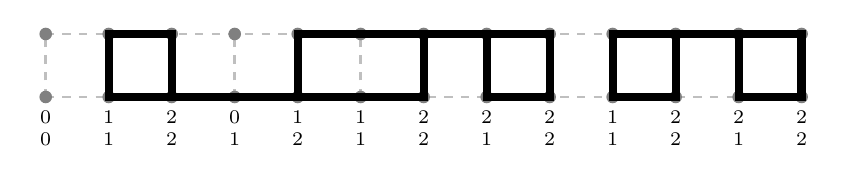
\begin{tikzpicture}[scale=0.8]
  \draw[gray!50, line width=1, dashed] (0,0) grid (12,1);
  \foreach \x in {0, 1, ..., 12} {
    \fill[gray]
      (\x,0) circle (0.1)
      (\x,1) circle (0.1)
    ;
  }
  \draw[line width=3, line cap=round]
    (1,0)--(1,1)--(2,1)--(2,0)--cycle
    (2,0)--(4,0)--(4,1)--(6,1)--(6,0)--(4,0)
    (6,1)--(8,1)--(8,0)--(7,0)--(7,1)
    % (4,1)--(6,1)--(6,0)--(8,0)--(8,1)--(6,1)
    % (2,1)--(4,1)--(4,0)--(2,0)
    % (4,1)--(5,1)--(5,0)--(8,0)--(8,1)--(7,1)--(7,0)
    (9,0) rectangle (10,1)--(11,1) rectangle (12,0);
  ;
  \node at (0,-0.5) {$\indx 00$};
  \node at (1,-0.5) {$\indx 11$};
  \node at (2,-0.5) {$\indx 22$};
  \node at (3,-0.5) {$\indx 01$};
  \node at (4,-0.5) {$\indx 12$};
  \node at (5,-0.5) {$\indx 11$};
  \node at (6,-0.5) {$\indx 22$};
  \node at (7,-0.5) {$\indx 21$};
  \node at (8,-0.5) {$\indx 22$};
  \node at (9,-0.5) {$\indx 11$};
  \node at (10,-0.5) {$\indx 22$};
  \node at (11,-0.5) {$\indx 21$};
  \node at (12,-0.5) {$\indx 22$};
\end{tikzpicture}
    \caption{An example of a leaf-free subgraph with its states labeled}
  \end{figure}
  \begin{figure}[ht!]
    \begin{align*}
  &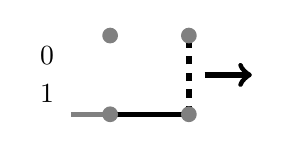
\begin{tikzpicture}[baseline=2.5ex]
    \draw[line width=2, line cap=round, white]
     (-1,0)--(0,0)
     (-1,1)--(0,1)
    ;
    \node at (-0.8,0.5) {$\indxxx 01$};
    \draw[line width=2, gray!100] (-0.5,0)--(0,0);
%
    \draw[line width=2] (0,0)--(1,0);
    \draw[line width=2, dashed] (1,0)--(1,1);
    \fill[gray] (0,0) circle (0.1) (1,0) circle (0.1) (0,1) circle (0.1) (1,1) circle (0.1);
%
    \draw[line width=2, ->] (1.2,0.5)--(1.8,0.5);
  \end{tikzpicture} \set{
  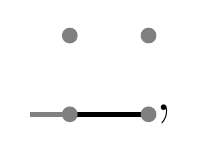
\begin{tikzpicture}[baseline=2.5ex]
    \draw[line width=2, gray!100] (-0.5,0)--(0,0);
    \draw[line width=2] (0,0)--(1,0);
%
    \fill[gray] (0,0) circle (0.1) (1,0) circle (0.1) (0,1) circle (0.1) (1,1) circle (0.1);
    \node at (1.2,0) {\Huge ,};
  \end{tikzpicture}
  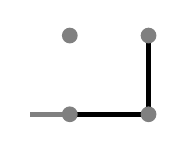
\begin{tikzpicture}[baseline=2.5ex]
    \draw[line width=2, gray!100] (-0.5,0)--(0,0);
%
    \draw[line width=2] (0,0)--(1,0);
    \draw[line width=2] (1,0)--(1,1);
    \fill[gray] (0,0) circle (0.1) (1,0) circle (0.1) (0,1) circle (0.1) (1,1) circle (0.1);
  \end{tikzpicture}
  }
  % = \set{\indxxx 12, \indxxx 01}
% Example 2
  \\
  &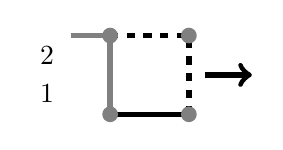
\begin{tikzpicture}[baseline=2.5ex]  % (2, 1) -> (0, 1), (1, 1), (1, 2), (2, 2)
      \draw[line width=2, line cap=round, white]
        (-1,0)--(0,0)
        (-1,1)--(0,1)
      ;
      \node at (-0.8,0.5) {$\indxxx 21$};
      \draw[line width=2, gray!100] (-0.5,1)--(0,1)--(0,0);
%
      \draw[line width=2] (0,0)--(1,0);
      \draw[line width=2, dashed] (0,1)--(1,1)--(1,0);
      \fill[gray] (0,0) circle (0.1) (1,0) circle (0.1) (0,1) circle (0.1) (1,1) circle (0.1);
    \draw[line width=2, ->] (1.2,0.5)--(1.8,0.5);
  \end{tikzpicture} \set{
  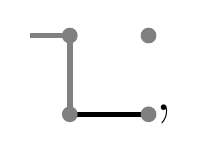
\begin{tikzpicture}[baseline=2.5ex]
    \draw[line width=2, gray!100] (-0.5,1)--(0,1)--(0,0);
    \draw[line width=2] (0,0)--(1,0);
%
    \fill[gray] (0,0) circle (0.1) (1,0) circle (0.1) (0,1) circle (0.1) (1,1) circle (0.1);
    \node at (1.2,0) {\Huge ,};
  \end{tikzpicture}
  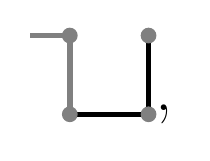
\begin{tikzpicture}[baseline=2.5ex]
    \draw[line width=2, gray!100] (-0.5,1)--(0,1)--(0,0);
    \draw[line width=2] (0,0)--(1,0)--(1,1);
%
    \fill[gray] (0,0) circle (0.1) (1,0) circle (0.1) (0,1) circle (0.1) (1,1) circle (0.1);
    \node at (1.2,0) {\Huge ,};
  \end{tikzpicture}
  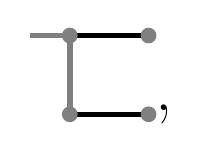
\begin{tikzpicture}[baseline=2.5ex]
    \draw[line width=2, gray!100] (-0.5,1)--(0,1)--(0,0);
    \draw[line width=2] (0,0)--(1,0) (0,1)--(1,1);
%
    \fill[gray] (0,0) circle (0.1) (1,0) circle (0.1) (0,1) circle (0.1) (1,1) circle (0.1);
    \node at (1.2,0) {\Huge ,};
  \end{tikzpicture}
  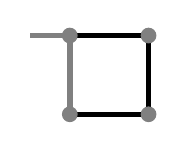
\begin{tikzpicture}[baseline=2.5ex]
    \draw[line width=2, gray!100] (-0.5,1)--(0,1)--(0,0);
    \draw[line width=2] (0,0)--(1,0)--(1,1)--(0,1);
%
    \fill[gray] (0,0) circle (0.1) (1,0) circle (0.1) (0,1) circle (0.1) (1,1) circle (0.1);
  \end{tikzpicture}
  }
\end{align*}
    \caption{Two examples of transitions from states to their children}
  \end{figure}
\end{frame}
%
\begin{frame}{Example: A System of Recurrences}
  The $1 \times 2$ grid has initial conditions
  \begin{align*}
    a_{\indxx 00}(1) &= a_{\indxx 11}(1) = 1 \\
    a_{\indxx 10}(1) &= a_{\indxx 01}(1) = a_{\indxx 12}(1) = a_{\indxx 21}(1) = a_{\indxx 22}(1) = 0,
  \end{align*}
  and satisfies the system of first order homogeneous difference relations
  \begin{align*}
    a_{\indxx 00}(n + 1) &= a_{\indxx 00}(n) + a_{\indxx 22}(n) \\
    a_{\indxx 01}(n + 1) &= a_{\indxx 01}(n) + a_{\indxx 21}(n) + a_{\indxx 22}(n) \\
    a_{\indxx 10}(n + 1) &= a_{\indxx 10}(n) + a_{\indxx 12}(n) + a_{\indxx 22}(n) \\
    a_{\indxx 11}(n + 1) &= a_{\indxx 00}(n) + a_{\indxx 11}(n) + a_{\indxx 12}(n)
                      + a_{\indxx 21}(n) + 2a_{\indxx 22}(n) \\
    a_{\indxx 12}(n + 1) &= a_{\indxx 01}(n) + a_{\indxx 21}(n) + a_{\indxx 22}(n) \\
    a_{\indxx 21}(n + 1) &= a_{\indxx 10}(n) + a_{\indxx 12}(n) + a_{\indxx 22}(n) \\
    a_{\indxx 22}(n + 1) &= a_{\indxx 11}(n) + a_{\indxx 12}(n) + a_{\indxx 21}(n) + a_{\indxx 22}(n).
  \end{align*}
\end{frame}

\begin{frame}{A single recurrence from a system of recurrences}
  \begin{theorem}[Corollary of Cayley–Hamilton theorem]
    In a system of first order homogeneous linear difference equations, \begin{align*}
      a^{(1)}(n+1) &= \alpha_{11}a^{(1)}(n) + \hdots + \alpha_{1k}a^{(k)}(n) \\
      \vdots\hspace{25pt} &= \hspace{66pt}\vdots  \\
      a^{(k)}(n+1) &= \alpha_{k1}a^{(1)}(n) + \hdots + \alpha_{kk}a^{(k)}(n)
    \end{align*} each equation satisfies the recurrence \[
      a^{(i)}(n) = -\beta_{k-1}a^{(i)}(n-1) - \hdots -\beta_{1}a^{(i)}(n-k-1) - \beta_0 a^{(i)}(n-k)
    \] for $n > k$ where $A = \{\alpha_{ij}\}_{i,j=1}^k$ is the coefficient matrix and \[
      m_A(x) = x^k + \beta_{k-1}x^{k-1} + \hdots + \beta_1 x + \beta_0
    \] is the minimal polynomial of $A$.
  \end{theorem}
\end{frame}

\begin{frame}{A single recurrence from a system of recurrences}
  \[
    \underbrace{\begin{bmatrix}
      a_{\indxx 00}(n) \\
      a_{\indxx 01}(n) \\
      a_{\indxx 10}(n) \\
      a_{\indxx 11}(n) \\
      a_{\indxx 12}(n) \\
      a_{\indxx 21}(n) \\
      a_{\indxx 22}(n)
    \end{bmatrix}}_{\vec a(n)}
    =
    \underbrace{\begin{bmatrix}
      1 & 0 & 0 & 0 & 0 & 0 & 1 \\ % 00
      0 & 1 & 0 & 0 & 0 & 1 & 1 \\ % 01
      0 & 0 & 1 & 0 & 1 & 0 & 1 \\ % 10
      1 & 0 & 0 & 1 & 1 & 1 & 2 \\ % 11
      0 & 1 & 0 & 0 & 0 & 1 & 1 \\ % 12
      0 & 0 & 1 & 0 & 1 & 0 & 1 \\ % 21
      0 & 0 & 0 & 1 & 1 & 1 & 1 \\ % 22
    \end{bmatrix}^{n-1}}_{A^{n-1}}
    \underbrace{\begin{bmatrix}
      1 \\ 0 \\ 0 \\ 1 \\ 0 \\ 0 \\ 0
    \end{bmatrix}}_{\vec a(1)}
  \]

  Let $x^k + \beta_{k-1}x^{k-1} + \hdots + \beta_1 x + \beta_0$
  be the minimal polynomial of $A$.
  Then \begin{alignat*}{6}
    &A^k    &          &= -\beta_{k-1}A^{k-1}          &&- \hdots &&- \beta_1 A                &&- \beta_0 \\
    &A^{n-1}&\vec a(1) &= -\beta_{k-1}A^{n-2}\vec a(1) &&- \hdots &&- \beta_1 A^{n-k}\vec a(1) &&- \beta_0 A^{n-k-1}\vec a(1) \\
    &       &\vec a(n) &= -\beta_{k-1}\vec a(n-1)      &&- \hdots && - \beta_1 \vec a(n-k+1)   &&- \beta_0 \vec a(n-k)
  \end{alignat*}
\end{frame}

\begin{frame}{Some conjectural recurrences}
  For $k = 3, 4, 5$, $a_k(n)$ the number of leaf-free subgraphs of the $n \times k$
  grid graph is conjectured to satisfy
  \begin{alignat*}{3}
    % A301976
    % I can prove this satisfies the five term recurrence
    %    a(n) = 13a(n-1) - 18a(n-2) - 14a(n-3) + 15a(n-4) + 5a(n-5)
    % which is divisible by the minimal polynomial of a coefficient matrix.
     a_3(n) &= 12a_3(n-1)  &&-     6a_3(n-2) &&-    20a_3(n-3) \\
           &-  5a_3(n-4)  && &&
    \\~\\
    % A320097
    a_4(n) &= 36a_4(n-1)  &&-     7a_4(n-2) &&-   201a_4(n-3) \\
           &+ 49a_4(n-4)  &&+    20a_4(n-5) &&-     5a_4(n-6) \\
    \\
    % A320099 % If a coefficient looks like it might be prime, it is.
    a_5(n) &=   103a_5(n-1) &&+  1063a_5(n-2) &&-  1873a_5(n-3) \\
           &- 20274a_5(n-4) &&+ 44071a_5(n-5) &&- 10365a_5(n-6) \\
           &- 20208a_5(n-7) &&+ 5959a_5(n-8)  &&+  2300a_5(n-9) \\
           &- 500a_5(n-10)  &&                &&
  \end{alignat*}
  For $k = 6$, this is the conjectured to be an $18$-order recurrence.
  % a(n) = 328       * a(n-1)
  %      + 9352      * a(n-2)
  %      - 73707     * a(n-3)
  %      - 1316926   * a(n-4)
  %      + 17899527  * a(n-5)
  %      - 86159484  * a(n-6)
  %      + 197347344 * a(n-7)
  %      - 189660665 * a(n-8)
  %      - 31064889  * a(n-9)
  %      + 181086417 * a(n-10)
  %      - 67203429  * a(n-11)
  %      - 44867092  * a(n-12)
  %      + 22863191  * a(n-13)
  %      + 3088843   * a(n-14)
  %      - 2085907   * a(n-15)
  %      - 14621     * a(n-16)
  %      + 54420     * a(n-17)
  %      - 3420      * a(n-18)
\end{frame}

\begin{frame}{Subgraphs which satisfy linear recurrences}
  \center{
  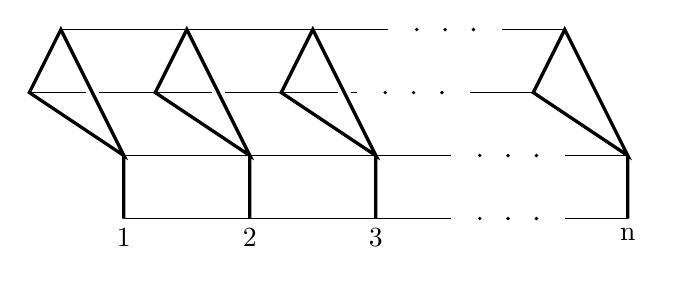
\begin{tikzpicture}[scale=0.8]
    \foreach \x in {0,2,4,8} {
      \draw[very thick] (\x + 2,-1)--(\x + 0.5,0)--(\x + 1,1)--cycle--(\x + 2,-2);
    }
    \draw
      (1,1)--(6.2,1) (8,1)--(9,1)
      (0.5,0)--(1.4,0) (1.6,0)--(3.4,0) (3.6,0)--(5.4,0) (5.6,0)--(5.7,0) (7.5,0)--(8.5,0)
      (2,-1)--(7.2,-1) (9,-1)--(10,-1)
      (2,-2)--(7.2,-2) (9,-2)--(10,-2)
    ;
    \fill
      (6.65, 1) circle (0.03) (7.10, 1) circle (0.03) (7.55, 1) circle (0.03)
      (6.15, 0) circle (0.03) (6.60, 0) circle (0.03) (7.05, 0) circle (0.03)
      (7.65, -1) circle (0.03) (8.10, -1) circle (0.03) (8.55, -1) circle (0.03)
      (7.65, -2) circle (0.03) (8.10, -2) circle (0.03) (8.55, -2) circle (0.03)
    ;
    \node[below] at (2,-2) {1};
    \node[below] at (4,-2) {2};
    \node[below] at (6,-2) {3};
    \node[below] at (10,-2) {n};
  \end{tikzpicture}
}
  \begin{theorem}[Faase, 1994] % https://www.researchgate.net/publication/2588839_On_the_number_of_specific_spanning_subgraphs_of_the_graphs_G_P_n
    Let $G$ be an arbitrary finite graph and let $H_n$ denote either the path
    graph $P_n$ or the cycle graph $C_n$ on $n$ vertices, and let $s(n)$
    count the number of subgraphs $S$ of the Cartesian product $G \square H_n$
    subject to any combination of the following properties:
    \begin{enumerate}
      \item Restrictions on degree
      \item Connectivity
      \item Acyclicity
    \end{enumerate}
    Then $s(n)$ satisfies a linear recurrence.
  \end{theorem}
\end{frame}

\begin{frame}{Examples: subgraphs which satisfy linear recurrences}
  Let $G_{n,k}$ be a grid graph, then the following classes of
  subgraphs satisfy linear recurrences:
  \begin{columns}
    \begin{column}{0.55\textwidth}
      \begin{itemize}
        \item Leaf-free subgraphs \begin{itemize}
          \item Degree set $D = \{0, 2, 3, 4\}$
        \end{itemize}
        \item Spanning tree (mazes) \begin{itemize}
          \item Degree set $D = \{1,2,3,4\}$
          \item Connected
          \item Acyclic
        \end{itemize}
      \end{itemize}
    \end{column}
    \begin{column}{0.45\textwidth}
      \begin{itemize}
        \item Hamiltonian paths \begin{itemize}
          \item Degree set $D = \{1, 2\}$
          \item Connected
          \item Acyclic
        \end{itemize}
        \item Perfect matchings (domino tilings) \begin{itemize}
          \item Degree set $D = \{1\}$
        \end{itemize}
      \end{itemize}
    \end{column}
  \end{columns}
  \begin{figure}[ht!]
    % Can we count this up to dihedral action?
    % Does there exist such a tree with >k leaves? This is NP-complete.
    %   (Maximum Leaf Spanning Tree Problem for Grid Graphs by Li)
    \center{
  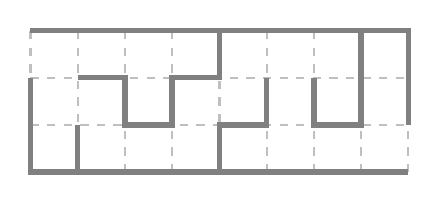
\begin{tikzpicture}[scale=0.6]
    \draw[thick, gray!50, dashed] (0,0) grid (8,3);
    \draw[line width=2, black!50]
      (0,2)--(0,0)--(8,0)
      (1,0)--(1,1)
      (0,3)--(0,3)--(4,3)--(4,2)--(3,2)--(3,1)--(2,1)--(2,2)--(1,2)
      (5,2)--(5,1)--(4,1)--(4,0)
      (8,1)--(8,3)--(0,3)
      (6,2)--(6,1)--(7,1)--(7,3)
    ;
  \end{tikzpicture}
  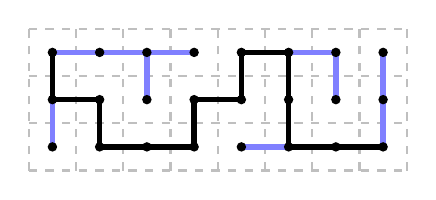
\begin{tikzpicture}[scale = 0.6]
    \draw[thick, gray!50, dashed] (0,4) grid (8,7);

    \draw[line width=2, blue!50]
      (7.5,4.5)--(7.5,6.5)
      (5.5,6.5)--(6.5,6.5)--(6.5,5.5)
      (5.5,4.5)--(4.5,4.5)
      (0.5,4.5)--(0.5,5.5)
      (0.5,6.5)--(3.5,6.5) (2.5,5.5)--(2.5,6.5)
    ;
    \draw[line width=2]
      (7.5,4.5)--(5.5,4.5)--(5.5,6.5)--(4.5,6.5)--(4.5,5.5)--(3.5,5.5)--
      (3.5,4.5)--(1.5,4.5)--(1.5,5.5)--(0.5,5.5)--(0.5,6.5)
    ;
    \foreach \x in {1,2,3} {
      \foreach \y in {0,1,...,7} {
        \fill (\y + 0.5, \x + 3.5) circle (0.1);
      }
    }
  \end{tikzpicture}
  }
    \caption{A correspondence between mazes and spanning trees}
  \end{figure}
\end{frame}

\begin{frame}{Generalizing domino tilings}

\end{frame}

\begin{frame}{More subgraphs which satisfy linear recurrences}
  \begin{theorem}
    Let $H$ be a group and $X$ be an arbitrary finite graph upon which $H$ acts.
    Then let $s(n)$ count the number of subsets of
    $X \square P_n$ subject to any combination of the following properties:
    \begin{enumerate}
      \item Exactly/fewer than/more than $m$ vertices of degree $d$
      \item Exactly/fewer than/more than $c$ connected components on
        exactly/fewer than/more than $d$ vertex.
      \item An odd/even number of vertices of degree $d$
      \item Exactly $\ell$ connected components
      \item Fixed by the induced action of $h \in H$
    \end{enumerate}
    Then $s(n)$ satisfies a linear recurrence.
  \end{theorem}
  % Example?
  \begin{corollary}
    The number of subgraphs of $X \square P_n$ (with appropriate vertex degree,
    connectivity, or acyclicity restrictions) counted up to the group action of
    $H$ satisfies a linear recurrence.
  \end{corollary}
\end{frame}

\begin{frame}{Up to horizontal/vertical reflection} % A303930
  The number of no-leaf subgraphs of the $2 \times n$ grid satisfies the two
  term recurrence \[
    a_2(n) = 5a_2(n-1) - 5a_2(n-2).
  \]

  The number of no-leaf subgraphs of the $2 \times n$ grid up to
  horizontal/vertical reflection is conjectured to satisfy the eight term
  recurrence
  \begin{align*}
    s(n) &= 8s(n-1) - 16s(n-2) - 20s(n-3) + 95s(n-4) \\
         &\hspace{1cm}- 60s(n-5) - 80s(n-6) + 100s(n-7) - 25s(n-8)
  \end{align*}
  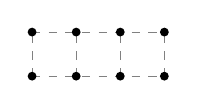
\begin{tikzpicture}[scale = 0.56]
  \draw[dashed,gray] (0,0) grid (3,1);
  \foreach \x in {0,1,2,3} {
    \fill (\x, 0) circle (0.1);
    \fill (\x, 1) circle (0.1);
  }
\end{tikzpicture}
~
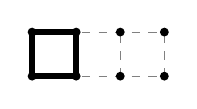
\begin{tikzpicture}[scale = 0.56]
  \draw[dashed,gray] (0,0) grid (3,1);
  \draw[line width = 2] (0,0) rectangle (1,1);
  \foreach \x in {0,1,2,3} {
    \fill (\x, 0) circle (0.1);
    \fill (\x, 1) circle (0.1);
  }
\end{tikzpicture}
~
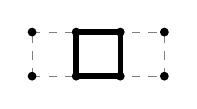
\begin{tikzpicture}[scale = 0.56]
  \draw[dashed,gray] (0,0) grid (3,1);
  \draw[line width = 2] (1,0) rectangle (2,1);
  \foreach \x in {0,1,2,3} {
    \fill (\x, 0) circle (0.1);
    \fill (\x, 1) circle (0.1);
  }
\end{tikzpicture}
~
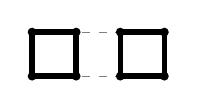
\begin{tikzpicture}[scale = 0.56]
  \draw[dashed,gray] (0,0) grid (3,1);
  \draw[line width = 2] (0,0) rectangle (1,1) (2,0) rectangle (3,1);
  \foreach \x in {0,1,2,3} {
    \fill (\x, 0) circle (0.1);
    \fill (\x, 1) circle (0.1);
  }
\end{tikzpicture}
~
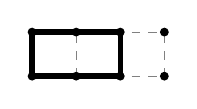
\begin{tikzpicture}[scale = 0.56]
  \draw[dashed,gray] (0,0) grid (3,1);
  \draw[line width = 2] (0,0) rectangle (2,1);
  \foreach \x in {0,1,2,3} {
    \fill (\x, 0) circle (0.1);
    \fill (\x, 1) circle (0.1);
  }
\end{tikzpicture}
\\~\\
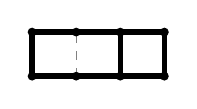
\begin{tikzpicture}[scale = 0.56]
  \draw[dashed,gray] (0,0) grid (3,1);
  \draw[line width = 2] (0,0) rectangle (2,1) rectangle (3,0);
  \foreach \x in {0,1,2,3} {
    \fill (\x, 0) circle (0.1);
    \fill (\x, 1) circle (0.1);
  }
\end{tikzpicture}
~
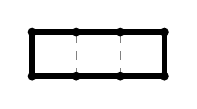
\begin{tikzpicture}[scale = 0.56]
  \draw[dashed,gray] (0,0) grid (3,1);
  \draw[line width = 2] (0,0) rectangle (3,1);
  \foreach \x in {0,1,2,3} {
    \fill (\x, 0) circle (0.1);
    \fill (\x, 1) circle (0.1);
  }
\end{tikzpicture}
~
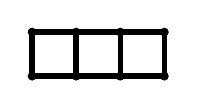
\begin{tikzpicture}[scale = 0.56]
  \draw[dashed,gray] (0,0) grid (3,1);
  \draw[line width = 2] (0,0) rectangle (1,1) rectangle (2,0) rectangle (3,1);
  \foreach \x in {0,1,2,3} {
    \fill (\x, 0) circle (0.1);
    \fill (\x, 1) circle (0.1);
  }
\end{tikzpicture}
~
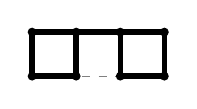
\begin{tikzpicture}[scale = 0.56]
  \draw[dashed,gray] (0,0) grid (3,1);
  \draw[line width = 2] (0,0) rectangle (1,1)--(2,1) rectangle (3,0);
  \foreach \x in {0,1,2,3} {
    \fill (\x, 0) circle (0.1);
    \fill (\x, 1) circle (0.1);
  }
\end{tikzpicture}
~
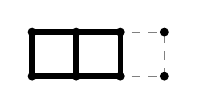
\begin{tikzpicture}[scale = 0.56]
  \draw[dashed,gray] (0,0) grid (3,1);
  \draw[line width = 2] (0,0) rectangle (1,1) rectangle (2,0);
  \foreach \x in {0,1,2,3} {
    \fill (\x, 0) circle (0.1);
    \fill (\x, 1) circle (0.1);
  }
\end{tikzpicture}
  % Eight term linear recurrence.
\end{frame}

\begin{frame}{Example: M\"obius ladder (Guy, 1967)}
  \begin{figure}
    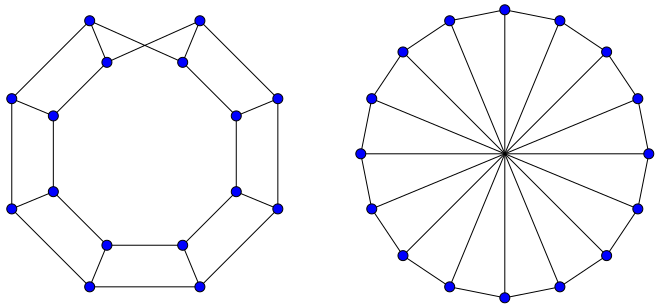
\includegraphics[width=240pt]{diagrams/Moebius-ladder-16.png}
    \caption{The M\"obius ladder $M_{16}$ on $16$ vertices.}
  \end{figure}
  \begin{fact}
    The number of leaf-free subgraphs on the M\"obius ladder on $2n$ vertices is
    equal to the number of leaf-free subgraphs on the $(n + 2) \times 2$ grid
    graph.
  \end{fact}
\end{frame}

\begin{frame}{Cycling around (a generalization of the M\"obius ladder)}
  \begin{theorem}
    Let $G$ be an arbitrary finite graph with vertex set
    $V = \{ v_1, v_2, \hdots, v_m \},$
    and let $E \subseteq V \times V$.
    Then let $H_n$ be the graph Cartesian product $G \square P_n$ together with
    the edges $\{((1, v_i), (n, v_j)) : (v_i, v_j) \in E\})$
    \\
    Next let $s(n)$ count the number of subgraphs of $H_n$
    subject to any combination of the following properties:
    \begin{enumerate}
      \item Restrictions on degree
      \item Connectivity
      \item Acyclicity
    \end{enumerate}
    Then $s(n)$ satisfies a linear recurrence.
  \end{theorem}
  Note that $E = \{(v_1, v_1), (v_2, v_2), \hdots, (v_m, v_m)\}$ recovers
  $G \square C_n$ and $E = \emptyset$ recovers $G \square P_n$.
\end{frame}

\begin{frame}{More exotic connections}
  \begin{theorem}
    Let $G$ be an arbitrary finite graph with vertex set
    $V = \{ v_1, v_2, \hdots, v_m \}$, and let $E \subseteq V \times V$.
    Then let $H_n$ be the disjoint union product
    $\underbrace{G \sqcup G \sqcup \hdots \sqcup G}_{n \text{ times}}$ together with the edges \[
      \{((k, v_i), (k + 1, v_j)) : (v_i, v_j) \in E, k \in [n-1]\}).
    \]
    Next let $s(n)$ count the number of subgraphs of $H_n$
    subject to any combination of the properties mentioned in the previous theorems.
    Then $s(n)$ satisfies a linear recurrence.
  \end{theorem}
  Note that $E = \{(v_1, v_1), (v_2, v_2), \hdots, (v_m, v_m)\}$ recovers
  $G \square P_n$.
\end{frame}

\begin{frame}{Example: king graph}
  Let $P_5$ be the path labeled $v_1, v_2, \hdots, v_5$ in the obvious way, and let
  $E = \set{(v_i, v_{i+i}) : i < 5} \cup \set{(v_i, v_{i}) : i \in [5]} \cup \set{(v_i, v_{i-i}) : i > 1}$.
  \begin{figure}
    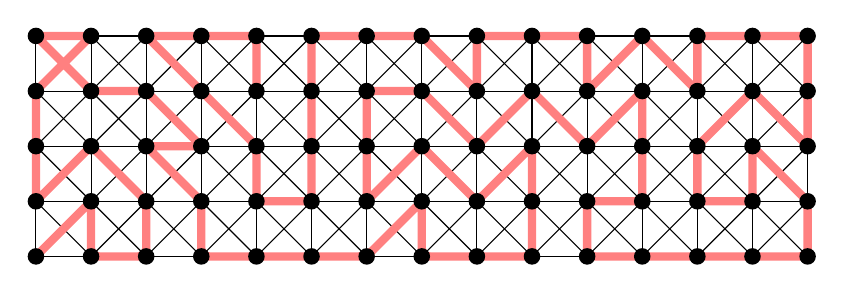
\begin{tikzpicture}[scale=0.7]
  \draw (0,0) grid (14,4);
  \foreach \x in {0,1,...,13} {
    \foreach \y in {0,1,2,3} {
      \draw (\x, \y)--(\x + 1, \y + 1);
      \draw (\x + 1, \y)--(\x, \y + 1);
    }
  }
  \draw[red!50, line width=3,rounded corners=1mm] (0,0)--(1,1)--(1,0)--(2,0)--(2,1)--(1,2)--(0,1)--(0,2)--(0,3)--(1,4)--(0,4)--(1,3)--(2,3)--(3,2)--(2,2)--(3,1)--(3,0)--(6,0)--(7,1)--(7,0)--(9,0)--(9,2)--(8,1)--(7,2)--(6,1)--(6,3)--(7,3)--(8,2)--(9,3)--(10,2)--(11,3)--(11,1)--(10,1)--(10,0)--(11,0)--(14,0)--(14,1)--(13,2)--(13,1)--(12,1)--(12,2)--(13,3)--(14,2)--(14,4)--(12,4)--(12,3)--(11,4)--(10,3)--(10,4)--(8,4)--(8,3)--(7,4)--(5,4)--(5,1)--(4,1)--(4,2)--(2,4)--(4,4)--(4,3);
  \foreach \x in {0,1,...,14} {
    \foreach \y in {0,1,...,4} {
      \fill (\x, \y) circle (0.15);
    }
  }
\end{tikzpicture}
    \caption{
      The number of ways a king can tour every square of the
      $5 \times 15$ chessboard is given by the number of Hamiltonian
      subgraphs in the $5 \times 15$ king graph
    }
  \end{figure}
  The number of kings tours on a $k \times n$ chessboard is a linear
  recurrence in $n$.
\end{frame}

\begin{frame}{Generalizations}
  \begin{itemize}
    \item Is there always a nice algorithm for counting subgraphs of the
      $n \times n$ grid graph satisfying particular properties?
      \begin{itemize}
        \item There are nice ways of counting domino tilings and spanning trees.
      \end{itemize}
    % \item It's sometimes faster to do, e.g. Kirchhoff's matrix tree theorem than count spanning trees this way.
    % \item (?) Can't count, say, acyclic orientations of G.
    % \item (?) Chromatic number exactly $2$ on $G \square P_n$?
    % \item Global properties: (e.g. no connected component is a shift of another connected component.)
    \item Given some graph and some properties, what is the order of recurrence
      that counts the number of subgraphs satisfying those properties?
  \end{itemize}

\end{frame}
\end{document}
